\documentclass[a4paper]{book}
\usepackage{a4wide}
\usepackage{makeidx}
\usepackage{fancyhdr}
\usepackage{graphicx}
\usepackage{multicol}
\usepackage{float}
\usepackage{textcomp}
\usepackage{alltt}
\usepackage{times}
\usepackage{ifpdf}
\ifpdf
\usepackage[pdftex,
            pagebackref=true,
            colorlinks=true,
            linkcolor=blue,
            unicode
           ]{hyperref}
\else
\usepackage[ps2pdf,
            pagebackref=true,
            colorlinks=true,
            linkcolor=blue,
            unicode
           ]{hyperref}
\usepackage{pspicture}
\fi
\usepackage[utf8]{inputenc}
\usepackage{doxygen}
\makeindex
\setcounter{tocdepth}{3}
\renewcommand{\footrulewidth}{0.4pt}
\begin{document}
\begin{titlepage}
\vspace*{7cm}
\begin{center}
{\Large kcl \\[1ex]\large 0.1 }\\
\vspace*{1cm}
{\large Generated by Doxygen 1.5.8}\\
\vspace*{0.5cm}
{\small Thu Sep 3 23:24:01 2009}\\
\end{center}
\end{titlepage}
\clearemptydoublepage
\pagenumbering{roman}
\tableofcontents
\clearemptydoublepage
\pagenumbering{arabic}
\chapter{Class Index}
\section{Class Hierarchy}
This inheritance list is sorted roughly, but not completely, alphabetically:\begin{CompactList}
\item \contentsline{section}{KGLBaseItem}{\pageref{class_k_g_l_base_item}}{}
\begin{CompactList}
\item \contentsline{section}{KGLItem}{\pageref{class_k_g_l_item}}{}
\begin{CompactList}
\item \contentsline{section}{KGLAnimItem}{\pageref{class_k_g_l_anim_item}}{}
\item \contentsline{section}{KGLBoxItem}{\pageref{class_k_g_l_box_item}}{}
\begin{CompactList}
\item \contentsline{section}{KGLPixmapItem}{\pageref{class_k_g_l_pixmap_item}}{}
\end{CompactList}
\item \contentsline{section}{KGLCircleItem}{\pageref{class_k_g_l_circle_item}}{}
\item \contentsline{section}{KGLContainerItem}{\pageref{class_k_g_l_container_item}}{}
\begin{CompactList}
\item \contentsline{section}{KGLIntroItem}{\pageref{class_k_g_l_intro_item}}{}
\end{CompactList}
\item \contentsline{section}{KGLGridItem}{\pageref{class_k_g_l_grid_item}}{}
\item \contentsline{section}{KGLParticlesItem}{\pageref{class_k_g_l_particles_item}}{}
\item \contentsline{section}{KGLPhysicsItem}{\pageref{class_k_g_l_physics_item}}{}
\item \contentsline{section}{KGLPolygonItem}{\pageref{class_k_g_l_polygon_item}}{}
\item \contentsline{section}{KGLShadowItem}{\pageref{class_k_g_l_shadow_item}}{}
\item \contentsline{section}{KGLShadowItem}{\pageref{class_k_g_l_shadow_item}}{}
\item \contentsline{section}{KGLTextItem}{\pageref{class_k_g_l_text_item}}{}
\end{CompactList}
\end{CompactList}
\item \contentsline{section}{KGLContactListener}{\pageref{class_k_g_l_contact_listener}}{}
\item \contentsline{section}{KGLEngine}{\pageref{class_k_g_l_engine}}{}
\begin{CompactList}
\item \contentsline{section}{KGLPhysicsEngine}{\pageref{class_k_g_l_physics_engine}}{}
\end{CompactList}
\item \contentsline{section}{KGLFx}{\pageref{class_k_g_l_fx}}{}
\begin{CompactList}
\item \contentsline{section}{KGLBlurFx}{\pageref{class_k_g_l_blur_fx}}{}
\item \contentsline{section}{KGLLightFx}{\pageref{class_k_g_l_light_fx}}{}
\item \contentsline{section}{KGLPixelateFx}{\pageref{class_k_g_l_pixelate_fx}}{}
\end{CompactList}
\item \contentsline{section}{KGLItemList}{\pageref{class_k_g_l_item_list}}{}
\item \contentsline{section}{KGLParticle}{\pageref{class_k_g_l_particle}}{}
\item \contentsline{section}{KGLPoint}{\pageref{class_k_g_l_point}}{}
\item \contentsline{section}{KGLPointList}{\pageref{class_k_g_l_point_list}}{}
\item \contentsline{section}{KGLProgram}{\pageref{class_k_g_l_program}}{}
\item \contentsline{section}{KGLScreenConfig}{\pageref{class_k_g_l_screen_config}}{}
\item \contentsline{section}{KGLShader}{\pageref{class_k_g_l_shader}}{}
\begin{CompactList}
\item \contentsline{section}{KGLFragmentShader}{\pageref{class_k_g_l_fragment_shader}}{}
\item \contentsline{section}{KGLVertexShader}{\pageref{class_k_g_l_vertex_shader}}{}
\end{CompactList}
\item \contentsline{section}{KGLTexture}{\pageref{class_k_g_l_texture}}{}
\item \contentsline{section}{KGLView}{\pageref{class_k_g_l_view}}{}
\end{CompactList}

\chapter{Class Index}
\section{Class List}
Here are the classes, structs, unions and interfaces with brief descriptions:\begin{CompactList}
\item\contentsline{section}{\hyperlink{class_abs_val}{AbsVal} }{\pageref{class_abs_val}}{}
\item\contentsline{section}{\hyperlink{class_k_c_l_code}{KCLCode} }{\pageref{class_k_c_l_code}}{}
\item\contentsline{section}{\hyperlink{class_k_c_l_device_model}{KCLDeviceModel} }{\pageref{class_k_c_l_device_model}}{}
\item\contentsline{section}{\hyperlink{class_k_c_l_engine}{KCLEngine} }{\pageref{class_k_c_l_engine}}{}
\item\contentsline{section}{\hyperlink{class_k_c_l_info_widget}{KCLInfoWidget} }{\pageref{class_k_c_l_info_widget}}{}
\item\contentsline{section}{\hyperlink{class_k_c_l_input}{KCLInput} (Provide an object that represent an input. This is the class mother of all device you want to use. It return you all information about the device, for example the name. And it return the status of the device, it means the type, code, and value )}{\pageref{class_k_c_l_input}}{}
\item\contentsline{section}{\hyperlink{class_k_c_l_input_event}{KCLInputEvent} (Provides a input events )}{\pageref{class_k_c_l_input_event}}{}
\item\contentsline{section}{\hyperlink{class_k_c_l_joystick}{KCLJoystick} }{\pageref{class_k_c_l_joystick}}{}
\item\contentsline{section}{\hyperlink{class_k_c_l_key_board}{KCLKeyBoard} }{\pageref{class_k_c_l_key_board}}{}
\item\contentsline{section}{\hyperlink{class_k_c_l_mouse}{KCLMouse} }{\pageref{class_k_c_l_mouse}}{}
\item\contentsline{section}{\hyperlink{class_k_c_l_thread}{KCLThread} (Provides a QThread witch listen the input status )}{\pageref{class_k_c_l_thread}}{}
\item\contentsline{section}{\hyperlink{class_virtual_button}{VirtualButton} }{\pageref{class_virtual_button}}{}
\end{CompactList}

\chapter{File Index}
\section{File List}
Here is a list of all files with brief descriptions:\begin{CompactList}
\item\contentsline{section}{/home/sacha/programmation/gluon/kal/\hyperlink{kalbuffer_8cpp}{kalbuffer.cpp} }{\pageref{kalbuffer_8cpp}}{}
\item\contentsline{section}{/home/sacha/programmation/gluon/kal/\hyperlink{kalbuffer_8h}{kalbuffer.h} }{\pageref{kalbuffer_8h}}{}
\item\contentsline{section}{/home/sacha/programmation/gluon/kal/\hyperlink{kalcapture_8cpp}{kalcapture.cpp} }{\pageref{kalcapture_8cpp}}{}
\item\contentsline{section}{/home/sacha/programmation/gluon/kal/\hyperlink{kalcapture_8h}{kalcapture.h} }{\pageref{kalcapture_8h}}{}
\item\contentsline{section}{/home/sacha/programmation/gluon/kal/\hyperlink{kalengine_8cpp}{kalengine.cpp} }{\pageref{kalengine_8cpp}}{}
\item\contentsline{section}{/home/sacha/programmation/gluon/kal/\hyperlink{kalengine_8h}{kalengine.h} }{\pageref{kalengine_8h}}{}
\item\contentsline{section}{/home/sacha/programmation/gluon/kal/\hyperlink{kalengine__export_8h}{kalengine\_\-export.h} }{\pageref{kalengine__export_8h}}{}
\item\contentsline{section}{/home/sacha/programmation/gluon/kal/\hyperlink{kalinfowidget_8cpp}{kalinfowidget.cpp} }{\pageref{kalinfowidget_8cpp}}{}
\item\contentsline{section}{/home/sacha/programmation/gluon/kal/\hyperlink{kalinfowidget_8h}{kalinfowidget.h} }{\pageref{kalinfowidget_8h}}{}
\item\contentsline{section}{/home/sacha/programmation/gluon/kal/\hyperlink{kaloggstreamer_8cpp}{kaloggstreamer.cpp} }{\pageref{kaloggstreamer_8cpp}}{}
\item\contentsline{section}{/home/sacha/programmation/gluon/kal/\hyperlink{kaloggstreamer_8h}{kaloggstreamer.h} }{\pageref{kaloggstreamer_8h}}{}
\item\contentsline{section}{/home/sacha/programmation/gluon/kal/\hyperlink{kalphonon_8cpp}{kalphonon.cpp} }{\pageref{kalphonon_8cpp}}{}
\item\contentsline{section}{/home/sacha/programmation/gluon/kal/\hyperlink{kalphonon_8h}{kalphonon.h} }{\pageref{kalphonon_8h}}{}
\item\contentsline{section}{/home/sacha/programmation/gluon/kal/\hyperlink{kalsoundloader_8cpp}{kalsoundloader.cpp} }{\pageref{kalsoundloader_8cpp}}{}
\item\contentsline{section}{/home/sacha/programmation/gluon/kal/\hyperlink{kalsoundloader_8h}{kalsoundloader.h} }{\pageref{kalsoundloader_8h}}{}
\item\contentsline{section}{/home/sacha/programmation/gluon/kal/\hyperlink{kalsource_8cpp}{kalsource.cpp} }{\pageref{kalsource_8cpp}}{}
\item\contentsline{section}{/home/sacha/programmation/gluon/kal/\hyperlink{kalsource_8h}{kalsource.h} }{\pageref{kalsource_8h}}{}
\end{CompactList}

\chapter{Class Documentation}
\hypertarget{class_abs_val}{
\section{AbsVal Class Reference}
\label{class_abs_val}\index{AbsVal@{AbsVal}}
}
{\tt \#include $<$kclinput.h$>$}

\subsection*{Public Member Functions}
\begin{CompactItemize}
\item 
\hyperlink{class_abs_val_1da0dbbce6fd776f580af9a149dfa21f}{AbsVal} (int v=0, int m=0, int M=0, int f=0, int F=0)
\end{CompactItemize}
\subsection*{Public Attributes}
\begin{CompactItemize}
\item 
int \hyperlink{class_abs_val_dea4f7aaaa630dc1e6784f3ce53294d6}{value}
\item 
int \hyperlink{class_abs_val_54069174e3b0dce6d75441750c2cb847}{min}
\item 
int \hyperlink{class_abs_val_e3764282970217b3f29827fe57da2a92}{max}
\item 
int \hyperlink{class_abs_val_87b40db59ddae36a643ca1a071b52116}{flat}
\item 
int \hyperlink{class_abs_val_872d15b6f387725daaaeb2e947a8ddde}{fuzz}
\end{CompactItemize}


\subsection{Constructor \& Destructor Documentation}
\hypertarget{class_abs_val_1da0dbbce6fd776f580af9a149dfa21f}{
\index{AbsVal@{AbsVal}!AbsVal@{AbsVal}}
\index{AbsVal@{AbsVal}!AbsVal@{AbsVal}}
\subsubsection[{AbsVal}]{\setlength{\rightskip}{0pt plus 5cm}AbsVal::AbsVal (int {\em v} = {\tt 0}, \/  int {\em m} = {\tt 0}, \/  int {\em M} = {\tt 0}, \/  int {\em f} = {\tt 0}, \/  int {\em F} = {\tt 0})\hspace{0.3cm}{\tt  \mbox{[}inline\mbox{]}}}}
\label{class_abs_val_1da0dbbce6fd776f580af9a149dfa21f}




\subsection{Member Data Documentation}
\hypertarget{class_abs_val_87b40db59ddae36a643ca1a071b52116}{
\index{AbsVal@{AbsVal}!flat@{flat}}
\index{flat@{flat}!AbsVal@{AbsVal}}
\subsubsection[{flat}]{\setlength{\rightskip}{0pt plus 5cm}int {\bf AbsVal::flat}}}
\label{class_abs_val_87b40db59ddae36a643ca1a071b52116}


\hypertarget{class_abs_val_872d15b6f387725daaaeb2e947a8ddde}{
\index{AbsVal@{AbsVal}!fuzz@{fuzz}}
\index{fuzz@{fuzz}!AbsVal@{AbsVal}}
\subsubsection[{fuzz}]{\setlength{\rightskip}{0pt plus 5cm}int {\bf AbsVal::fuzz}}}
\label{class_abs_val_872d15b6f387725daaaeb2e947a8ddde}


\hypertarget{class_abs_val_e3764282970217b3f29827fe57da2a92}{
\index{AbsVal@{AbsVal}!max@{max}}
\index{max@{max}!AbsVal@{AbsVal}}
\subsubsection[{max}]{\setlength{\rightskip}{0pt plus 5cm}int {\bf AbsVal::max}}}
\label{class_abs_val_e3764282970217b3f29827fe57da2a92}


\hypertarget{class_abs_val_54069174e3b0dce6d75441750c2cb847}{
\index{AbsVal@{AbsVal}!min@{min}}
\index{min@{min}!AbsVal@{AbsVal}}
\subsubsection[{min}]{\setlength{\rightskip}{0pt plus 5cm}int {\bf AbsVal::min}}}
\label{class_abs_val_54069174e3b0dce6d75441750c2cb847}


\hypertarget{class_abs_val_dea4f7aaaa630dc1e6784f3ce53294d6}{
\index{AbsVal@{AbsVal}!value@{value}}
\index{value@{value}!AbsVal@{AbsVal}}
\subsubsection[{value}]{\setlength{\rightskip}{0pt plus 5cm}int {\bf AbsVal::value}}}
\label{class_abs_val_dea4f7aaaa630dc1e6784f3ce53294d6}




The documentation for this class was generated from the following file:\begin{CompactItemize}
\item 
/home/sacha/programmation/gluon/kcl/\hyperlink{kclinput_8h}{kclinput.h}\end{CompactItemize}

\hypertarget{class_k_c_l_code}{
\section{KCLCode Class Reference}
\label{class_k_c_l_code}\index{KCLCode@{KCLCode}}
}
{\tt \#include $<$kclcode.h$>$}

\subsection*{Static Public Member Functions}
\begin{CompactItemize}
\item 
static QString \hyperlink{class_k_c_l_code_2b4ae042dbc8622b23bc025506aff9af}{keyName} (int code)
\item 
static QString \hyperlink{class_k_c_l_code_220faab8799839c0990bfab94921fef0}{eventName} (int code)
\item 
static QString \hyperlink{class_k_c_l_code_8d559916777d0147c8863b869392004a}{relativName} (int code)
\item 
static QString \hyperlink{class_k_c_l_code_9b4daee151b687abef17c9600a43dec3}{absoluName} (int code)
\end{CompactItemize}


\subsection{Member Function Documentation}
\hypertarget{class_k_c_l_code_9b4daee151b687abef17c9600a43dec3}{
\index{KCLCode@{KCLCode}!absoluName@{absoluName}}
\index{absoluName@{absoluName}!KCLCode@{KCLCode}}
\subsubsection[{absoluName}]{\setlength{\rightskip}{0pt plus 5cm}QString KCLCode::absoluName (int {\em code})\hspace{0.3cm}{\tt  \mbox{[}static\mbox{]}}}}
\label{class_k_c_l_code_9b4daee151b687abef17c9600a43dec3}


\hypertarget{class_k_c_l_code_220faab8799839c0990bfab94921fef0}{
\index{KCLCode@{KCLCode}!eventName@{eventName}}
\index{eventName@{eventName}!KCLCode@{KCLCode}}
\subsubsection[{eventName}]{\setlength{\rightskip}{0pt plus 5cm}static QString KCLCode::eventName (int {\em code})\hspace{0.3cm}{\tt  \mbox{[}static\mbox{]}}}}
\label{class_k_c_l_code_220faab8799839c0990bfab94921fef0}


\hypertarget{class_k_c_l_code_2b4ae042dbc8622b23bc025506aff9af}{
\index{KCLCode@{KCLCode}!keyName@{keyName}}
\index{keyName@{keyName}!KCLCode@{KCLCode}}
\subsubsection[{keyName}]{\setlength{\rightskip}{0pt plus 5cm}QString KCLCode::keyName (int {\em code})\hspace{0.3cm}{\tt  \mbox{[}static\mbox{]}}}}
\label{class_k_c_l_code_2b4ae042dbc8622b23bc025506aff9af}


\hypertarget{class_k_c_l_code_8d559916777d0147c8863b869392004a}{
\index{KCLCode@{KCLCode}!relativName@{relativName}}
\index{relativName@{relativName}!KCLCode@{KCLCode}}
\subsubsection[{relativName}]{\setlength{\rightskip}{0pt plus 5cm}QString KCLCode::relativName (int {\em code})\hspace{0.3cm}{\tt  \mbox{[}static\mbox{]}}}}
\label{class_k_c_l_code_8d559916777d0147c8863b869392004a}




The documentation for this class was generated from the following files:\begin{CompactItemize}
\item 
/home/sacha/programmation/gluon/kcl/\hyperlink{kclcode_8h}{kclcode.h}\item 
/home/sacha/programmation/gluon/kcl/\hyperlink{kclcode_8cpp}{kclcode.cpp}\end{CompactItemize}

\hypertarget{class_k_c_l_device_model}{
\section{KCLDeviceModel Class Reference}
\label{class_k_c_l_device_model}\index{KCLDeviceModel@{KCLDeviceModel}}
}
{\tt \#include $<$kcldevicemodel.h$>$}

\subsection*{Public Member Functions}
\begin{CompactItemize}
\item 
\hyperlink{class_k_c_l_device_model_4015fbee857e468d75861e2aa13e5653}{KCLDeviceModel} (QObject $\ast$parent=0)
\item 
void \hyperlink{class_k_c_l_device_model_ed625ef5cc19fc60dfc92861b64d9656}{setupList} ()
\item 
void \hyperlink{class_k_c_l_device_model_b9f26d59942f74cf73605a7d1a445c2d}{addLine} (QString text, KIcon icon, \hyperlink{kclinput_8h_833b28f90e109607cd5d9e826474893a}{DEVICE} device)
\end{CompactItemize}


\subsection{Constructor \& Destructor Documentation}
\hypertarget{class_k_c_l_device_model_4015fbee857e468d75861e2aa13e5653}{
\index{KCLDeviceModel@{KCLDeviceModel}!KCLDeviceModel@{KCLDeviceModel}}
\index{KCLDeviceModel@{KCLDeviceModel}!KCLDeviceModel@{KCLDeviceModel}}
\subsubsection[{KCLDeviceModel}]{\setlength{\rightskip}{0pt plus 5cm}KCLDeviceModel::KCLDeviceModel (QObject $\ast$ {\em parent} = {\tt 0})}}
\label{class_k_c_l_device_model_4015fbee857e468d75861e2aa13e5653}




\subsection{Member Function Documentation}
\hypertarget{class_k_c_l_device_model_b9f26d59942f74cf73605a7d1a445c2d}{
\index{KCLDeviceModel@{KCLDeviceModel}!addLine@{addLine}}
\index{addLine@{addLine}!KCLDeviceModel@{KCLDeviceModel}}
\subsubsection[{addLine}]{\setlength{\rightskip}{0pt plus 5cm}void KCLDeviceModel::addLine (QString {\em text}, \/  KIcon {\em icon}, \/  {\bf DEVICE} {\em device})}}
\label{class_k_c_l_device_model_b9f26d59942f74cf73605a7d1a445c2d}


\hypertarget{class_k_c_l_device_model_ed625ef5cc19fc60dfc92861b64d9656}{
\index{KCLDeviceModel@{KCLDeviceModel}!setupList@{setupList}}
\index{setupList@{setupList}!KCLDeviceModel@{KCLDeviceModel}}
\subsubsection[{setupList}]{\setlength{\rightskip}{0pt plus 5cm}void KCLDeviceModel::setupList ()}}
\label{class_k_c_l_device_model_ed625ef5cc19fc60dfc92861b64d9656}




The documentation for this class was generated from the following files:\begin{CompactItemize}
\item 
/home/sacha/programmation/gluon/kcl/\hyperlink{kcldevicemodel_8h}{kcldevicemodel.h}\item 
/home/sacha/programmation/gluon/kcl/\hyperlink{kcldevicemodel_8cpp}{kcldevicemodel.cpp}\end{CompactItemize}

\hypertarget{class_k_c_l_engine}{
\section{KCLEngine Class Reference}
\label{class_k_c_l_engine}\index{KCLEngine@{KCLEngine}}
}
{\tt \#include $<$kclengine.h$>$}

\subsection*{Public Member Functions}
\begin{CompactItemize}
\item 
\hyperlink{class_k_c_l_engine_fbe8d629ee92a2611f9971ed1bb718f3}{KCLEngine} (QObject $\ast$parent=0)
\item 
void \hyperlink{class_k_c_l_engine_20f234eb6e418964d9d2d8e1b9332f4f}{addInput} (\hyperlink{class_k_c_l_input}{KCLInput} $\ast$input)
\item 
void \hyperlink{class_k_c_l_engine_f72512ac8f67ae93805301da15146b8d}{addInput} (const QString \&deviceName)
\item 
void \hyperlink{class_k_c_l_engine_ef5bcdd289dcc543c61205707a1f39f1}{addInput} (\hyperlink{kclinput_8h_833b28f90e109607cd5d9e826474893a}{DEVICE} device, int id=0)
\item 
void \hyperlink{class_k_c_l_engine_f5f9dc8d3add7c53c27a9e5bbad7fef3}{remInput} (\hyperlink{class_k_c_l_input}{KCLInput} $\ast$input)
\item 
void \hyperlink{class_k_c_l_engine_5f138c0986344f0c8bec3f9374e2d122}{remInput} (\hyperlink{kclinput_8h_833b28f90e109607cd5d9e826474893a}{DEVICE} device, int id=0)
\item 
\hyperlink{class_k_c_l_input}{KCLInput} $\ast$ \hyperlink{class_k_c_l_engine_7e4af493818ecd2095325fe28d8db227}{input} (int id=0)
\item 
void \hyperlink{class_k_c_l_engine_886715d09ab70063e43ed63022c04345}{setButton} (QString name, int code, \hyperlink{class_k_c_l_input}{KCLInput} $\ast$input)
\item 
void \hyperlink{class_k_c_l_engine_265a2d0e58a5cd9c872c125bd95a47cb}{remAll} ()
\item 
void \hyperlink{class_k_c_l_engine_2d77246e1d5c194dd224e2f0e7bff05e}{searchDevice} ()
\item 
bool \hyperlink{class_k_c_l_engine_0bcbf5200cdbf84b6e73b804e5064836}{button} (QString name)
\item 
bool \hyperlink{class_k_c_l_engine_aff35dae398c148743797b774d14647a}{anyPress} ()
\item 
bool \hyperlink{class_k_c_l_engine_1dd1ac1227dc51b3244205cf40ab105a}{anyMove} ()
\item 
QStringList \hyperlink{class_k_c_l_engine_7b3834bd74520513874137bb785c027f}{deviceList} (\hyperlink{kclinput_8h_833b28f90e109607cd5d9e826474893a}{DEVICE} device)
\end{CompactItemize}


\subsection{Constructor \& Destructor Documentation}
\hypertarget{class_k_c_l_engine_fbe8d629ee92a2611f9971ed1bb718f3}{
\index{KCLEngine@{KCLEngine}!KCLEngine@{KCLEngine}}
\index{KCLEngine@{KCLEngine}!KCLEngine@{KCLEngine}}
\subsubsection[{KCLEngine}]{\setlength{\rightskip}{0pt plus 5cm}KCLEngine::KCLEngine (QObject $\ast$ {\em parent} = {\tt 0})}}
\label{class_k_c_l_engine_fbe8d629ee92a2611f9971ed1bb718f3}




\subsection{Member Function Documentation}
\hypertarget{class_k_c_l_engine_ef5bcdd289dcc543c61205707a1f39f1}{
\index{KCLEngine@{KCLEngine}!addInput@{addInput}}
\index{addInput@{addInput}!KCLEngine@{KCLEngine}}
\subsubsection[{addInput}]{\setlength{\rightskip}{0pt plus 5cm}void KCLEngine::addInput ({\bf DEVICE} {\em device}, \/  int {\em id} = {\tt 0})}}
\label{class_k_c_l_engine_ef5bcdd289dcc543c61205707a1f39f1}


\hypertarget{class_k_c_l_engine_f72512ac8f67ae93805301da15146b8d}{
\index{KCLEngine@{KCLEngine}!addInput@{addInput}}
\index{addInput@{addInput}!KCLEngine@{KCLEngine}}
\subsubsection[{addInput}]{\setlength{\rightskip}{0pt plus 5cm}void KCLEngine::addInput (const QString \& {\em deviceName})}}
\label{class_k_c_l_engine_f72512ac8f67ae93805301da15146b8d}


\hypertarget{class_k_c_l_engine_20f234eb6e418964d9d2d8e1b9332f4f}{
\index{KCLEngine@{KCLEngine}!addInput@{addInput}}
\index{addInput@{addInput}!KCLEngine@{KCLEngine}}
\subsubsection[{addInput}]{\setlength{\rightskip}{0pt plus 5cm}void KCLEngine::addInput ({\bf KCLInput} $\ast$ {\em input})}}
\label{class_k_c_l_engine_20f234eb6e418964d9d2d8e1b9332f4f}


\hypertarget{class_k_c_l_engine_1dd1ac1227dc51b3244205cf40ab105a}{
\index{KCLEngine@{KCLEngine}!anyMove@{anyMove}}
\index{anyMove@{anyMove}!KCLEngine@{KCLEngine}}
\subsubsection[{anyMove}]{\setlength{\rightskip}{0pt plus 5cm}bool KCLEngine::anyMove ()}}
\label{class_k_c_l_engine_1dd1ac1227dc51b3244205cf40ab105a}


\hypertarget{class_k_c_l_engine_aff35dae398c148743797b774d14647a}{
\index{KCLEngine@{KCLEngine}!anyPress@{anyPress}}
\index{anyPress@{anyPress}!KCLEngine@{KCLEngine}}
\subsubsection[{anyPress}]{\setlength{\rightskip}{0pt plus 5cm}bool KCLEngine::anyPress ()}}
\label{class_k_c_l_engine_aff35dae398c148743797b774d14647a}


\hypertarget{class_k_c_l_engine_0bcbf5200cdbf84b6e73b804e5064836}{
\index{KCLEngine@{KCLEngine}!button@{button}}
\index{button@{button}!KCLEngine@{KCLEngine}}
\subsubsection[{button}]{\setlength{\rightskip}{0pt plus 5cm}bool KCLEngine::button (QString {\em name})}}
\label{class_k_c_l_engine_0bcbf5200cdbf84b6e73b804e5064836}


\hypertarget{class_k_c_l_engine_7b3834bd74520513874137bb785c027f}{
\index{KCLEngine@{KCLEngine}!deviceList@{deviceList}}
\index{deviceList@{deviceList}!KCLEngine@{KCLEngine}}
\subsubsection[{deviceList}]{\setlength{\rightskip}{0pt plus 5cm}QStringList KCLEngine::deviceList ({\bf DEVICE} {\em device})\hspace{0.3cm}{\tt  \mbox{[}inline\mbox{]}}}}
\label{class_k_c_l_engine_7b3834bd74520513874137bb785c027f}


\hypertarget{class_k_c_l_engine_7e4af493818ecd2095325fe28d8db227}{
\index{KCLEngine@{KCLEngine}!input@{input}}
\index{input@{input}!KCLEngine@{KCLEngine}}
\subsubsection[{input}]{\setlength{\rightskip}{0pt plus 5cm}{\bf KCLInput}$\ast$ KCLEngine::input (int {\em id} = {\tt 0})\hspace{0.3cm}{\tt  \mbox{[}inline\mbox{]}}}}
\label{class_k_c_l_engine_7e4af493818ecd2095325fe28d8db227}


\hypertarget{class_k_c_l_engine_265a2d0e58a5cd9c872c125bd95a47cb}{
\index{KCLEngine@{KCLEngine}!remAll@{remAll}}
\index{remAll@{remAll}!KCLEngine@{KCLEngine}}
\subsubsection[{remAll}]{\setlength{\rightskip}{0pt plus 5cm}void KCLEngine::remAll ()}}
\label{class_k_c_l_engine_265a2d0e58a5cd9c872c125bd95a47cb}


\hypertarget{class_k_c_l_engine_5f138c0986344f0c8bec3f9374e2d122}{
\index{KCLEngine@{KCLEngine}!remInput@{remInput}}
\index{remInput@{remInput}!KCLEngine@{KCLEngine}}
\subsubsection[{remInput}]{\setlength{\rightskip}{0pt plus 5cm}void KCLEngine::remInput ({\bf DEVICE} {\em device}, \/  int {\em id} = {\tt 0})}}
\label{class_k_c_l_engine_5f138c0986344f0c8bec3f9374e2d122}


\hypertarget{class_k_c_l_engine_f5f9dc8d3add7c53c27a9e5bbad7fef3}{
\index{KCLEngine@{KCLEngine}!remInput@{remInput}}
\index{remInput@{remInput}!KCLEngine@{KCLEngine}}
\subsubsection[{remInput}]{\setlength{\rightskip}{0pt plus 5cm}void KCLEngine::remInput ({\bf KCLInput} $\ast$ {\em input})\hspace{0.3cm}{\tt  \mbox{[}inline\mbox{]}}}}
\label{class_k_c_l_engine_f5f9dc8d3add7c53c27a9e5bbad7fef3}


\hypertarget{class_k_c_l_engine_2d77246e1d5c194dd224e2f0e7bff05e}{
\index{KCLEngine@{KCLEngine}!searchDevice@{searchDevice}}
\index{searchDevice@{searchDevice}!KCLEngine@{KCLEngine}}
\subsubsection[{searchDevice}]{\setlength{\rightskip}{0pt plus 5cm}void KCLEngine::searchDevice ()}}
\label{class_k_c_l_engine_2d77246e1d5c194dd224e2f0e7bff05e}


\hypertarget{class_k_c_l_engine_886715d09ab70063e43ed63022c04345}{
\index{KCLEngine@{KCLEngine}!setButton@{setButton}}
\index{setButton@{setButton}!KCLEngine@{KCLEngine}}
\subsubsection[{setButton}]{\setlength{\rightskip}{0pt plus 5cm}void KCLEngine::setButton (QString {\em name}, \/  int {\em code}, \/  {\bf KCLInput} $\ast$ {\em input})}}
\label{class_k_c_l_engine_886715d09ab70063e43ed63022c04345}




The documentation for this class was generated from the following files:\begin{CompactItemize}
\item 
/home/sacha/programmation/gluon/kcl/\hyperlink{kclengine_8h}{kclengine.h}\item 
/home/sacha/programmation/gluon/kcl/\hyperlink{kclengine_8cpp}{kclengine.cpp}\end{CompactItemize}

\hypertarget{class_k_c_l_info_widget}{
\section{KCLInfoWidget Class Reference}
\label{class_k_c_l_info_widget}\index{KCLInfoWidget@{KCLInfoWidget}}
}
{\tt \#include $<$kclinfowidget.h$>$}

\subsection*{Public Member Functions}
\begin{CompactItemize}
\item 
\hyperlink{class_k_c_l_info_widget_2114f10ac40847ddafb03d19bebef203}{KCLInfoWidget} (QWidget $\ast$parent=0)
\end{CompactItemize}


\subsection{Constructor \& Destructor Documentation}
\hypertarget{class_k_c_l_info_widget_2114f10ac40847ddafb03d19bebef203}{
\index{KCLInfoWidget@{KCLInfoWidget}!KCLInfoWidget@{KCLInfoWidget}}
\index{KCLInfoWidget@{KCLInfoWidget}!KCLInfoWidget@{KCLInfoWidget}}
\subsubsection[{KCLInfoWidget}]{\setlength{\rightskip}{0pt plus 5cm}KCLInfoWidget::KCLInfoWidget (QWidget $\ast$ {\em parent} = {\tt 0})}}
\label{class_k_c_l_info_widget_2114f10ac40847ddafb03d19bebef203}




The documentation for this class was generated from the following files:\begin{CompactItemize}
\item 
/home/sacha/programmation/gluon/kcl/\hyperlink{kclinfowidget_8h}{kclinfowidget.h}\item 
/home/sacha/programmation/gluon/kcl/\hyperlink{kclinfowidget_8cpp}{kclinfowidget.cpp}\end{CompactItemize}

\hypertarget{class_k_c_l_input}{
\section{KCLInput Class Reference}
\label{class_k_c_l_input}\index{KCLInput@{KCLInput}}
}
provide an object that represent an input. This is the class mother of all device you want to use. It return you all information about the device, for example the name. And it return the status of the device, it means the type, code, and value.  


{\tt \#include $<$Gluon/KCL/KCLInput$>$}

Inheritance diagram for KCLInput::\begin{figure}[H]
\begin{center}
\leavevmode
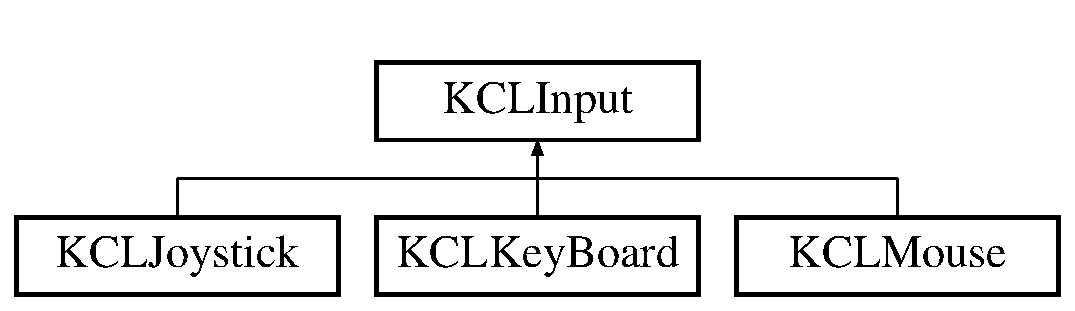
\includegraphics[height=2cm]{class_k_c_l_input}
\end{center}
\end{figure}
\subsection*{Public Slots}
\begin{CompactItemize}
\item 
void \hyperlink{class_k_c_l_input_09e6f283721d38bb9aa2a703d6a735c6}{slotInputEvent} (\hyperlink{class_k_c_l_input_event}{KCLInputEvent} $\ast$event)
\end{CompactItemize}
\subsection*{Public Member Functions}
\begin{CompactItemize}
\item 
\hyperlink{class_k_c_l_input_8be2188910f86e335d36694068eab677}{KCLInput} (const QString \&device, QObject $\ast$parent=0)
\item 
\hyperlink{class_k_c_l_input_aea38929accc31d9f27c08b5d4119fe3}{$\sim$KCLInput} ()
\item 
unsigned int \hyperlink{class_k_c_l_input_8b974c847387834722f09ac5725f3c68}{vendor} ()
\item 
unsigned int \hyperlink{class_k_c_l_input_89c31b5c39e1f052d3408cb34861be51}{product} ()
\item 
unsigned int \hyperlink{class_k_c_l_input_53ebfb56b5039bdeb8b6bed4bbff1b0e}{version} ()
\item 
unsigned int \hyperlink{class_k_c_l_input_5636bb74f7e17ad8b09dcbbc3be2a736}{bustype} ()
\item 
QString \hyperlink{class_k_c_l_input_99047eea6d01d09f72a49dd219ce44e9}{device} ()
\item 
QString \hyperlink{class_k_c_l_input_0214f0e500c4eccdb7afacaf78019b14}{name} ()
\item 
\hyperlink{kclinput_8h_833b28f90e109607cd5d9e826474893a}{DEVICE} \hyperlink{class_k_c_l_input_cbbc1f4e0b0e7869d88173603f2f0c68}{deviceType} ()
\item 
bool \hyperlink{class_k_c_l_input_afe120b671d76b4b7d14b48e03d4faf6}{button} (int code)
\item 
bool \hyperlink{class_k_c_l_input_c3740f546a1992b7855549405c81dc7b}{anyPress} ()
\item 
bool \hyperlink{class_k_c_l_input_28b17185d4d20c96ef67a7bc287f5908}{anyMove} ()
\item 
int \hyperlink{class_k_c_l_input_80bd12aea5ae92a327af1db942ef25b9}{axisPosition} (int code)
\item 
int \hyperlink{class_k_c_l_input_5546e3862c917d07b22543190659871d}{axisAbsolu} (int code)
\item 
QList$<$ int $>$ \hyperlink{class_k_c_l_input_ae4174869c6bf29b6c59afa58c718275}{buttonCapabilities} ()
\item 
\hyperlink{class_abs_val}{AbsVal} \hyperlink{class_k_c_l_input_72c70fa38d90216025a913a1255ce935}{axisCapability} (int axisCode)
\item 
bool \hyperlink{class_k_c_l_input_0c3b7dd3cce5d5567c4894500074fee3}{error} ()
\item 
virtual void \hyperlink{class_k_c_l_input_ee93fa33ec6a14baf2acf3daf23607c0}{inputEventFilter} (\hyperlink{class_k_c_l_input_event}{KCLInputEvent} $\ast$event)
\end{CompactItemize}
\subsection*{Protected Member Functions}
\begin{CompactItemize}
\item 
void \hyperlink{class_k_c_l_input_33e1fd26c084040a728cabf03e445893}{readInformation} ()
\end{CompactItemize}


\subsection{Detailed Description}
provide an object that represent an input. This is the class mother of all device you want to use. It return you all information about the device, for example the name. And it return the status of the device, it means the type, code, and value. 

\begin{Desc}
\item[Author:]sacha schutz $<$\href{mailto:istdasklar@gmail.com}{\tt istdasklar@gmail.com}$>$\end{Desc}
\hypertarget{class_k_c_l_input_creating}{}\subsection{Creating a KCLInput}\label{class_k_c_l_input_creating}
The easiest way to create usable \hyperlink{class_k_c_l_input}{KCLInput} is to set it by the evdev file name. 

\begin{Code}\begin{verbatim} KCLInput * myInput  = new KCLInput("/dev/input/event2");
 kDebug()<<myInput->name();
\end{verbatim}
\end{Code}

 

\subsection{Constructor \& Destructor Documentation}
\hypertarget{class_k_c_l_input_8be2188910f86e335d36694068eab677}{
\index{KCLInput@{KCLInput}!KCLInput@{KCLInput}}
\index{KCLInput@{KCLInput}!KCLInput@{KCLInput}}
\subsubsection[{KCLInput}]{\setlength{\rightskip}{0pt plus 5cm}KCLInput::KCLInput (const QString \& {\em device}, \/  QObject $\ast$ {\em parent} = {\tt 0})}}
\label{class_k_c_l_input_8be2188910f86e335d36694068eab677}


\hypertarget{class_k_c_l_input_aea38929accc31d9f27c08b5d4119fe3}{
\index{KCLInput@{KCLInput}!$\sim$KCLInput@{$\sim$KCLInput}}
\index{$\sim$KCLInput@{$\sim$KCLInput}!KCLInput@{KCLInput}}
\subsubsection[{$\sim$KCLInput}]{\setlength{\rightskip}{0pt plus 5cm}KCLInput::$\sim$KCLInput ()\hspace{0.3cm}{\tt  \mbox{[}inline\mbox{]}}}}
\label{class_k_c_l_input_aea38929accc31d9f27c08b5d4119fe3}




\subsection{Member Function Documentation}
\hypertarget{class_k_c_l_input_28b17185d4d20c96ef67a7bc287f5908}{
\index{KCLInput@{KCLInput}!anyMove@{anyMove}}
\index{anyMove@{anyMove}!KCLInput@{KCLInput}}
\subsubsection[{anyMove}]{\setlength{\rightskip}{0pt plus 5cm}bool KCLInput::anyMove ()\hspace{0.3cm}{\tt  \mbox{[}inline\mbox{]}}}}
\label{class_k_c_l_input_28b17185d4d20c96ef67a7bc287f5908}


\begin{Desc}
\item[Returns:]true if a motion is done by a motion input.( mouse , joystick ...) 

\begin{Code}\begin{verbatim} KCLInput * myInput = new KCLInput("/dev/input/event3");
 if ( myInput->anyMove()) kDebug()<<"you have move something...";
\end{verbatim}
\end{Code}

 \end{Desc}
\begin{Desc}
\item[See also:]\hyperlink{class_k_c_l_input_event}{KCLInputEvent} \end{Desc}
\hypertarget{class_k_c_l_input_c3740f546a1992b7855549405c81dc7b}{
\index{KCLInput@{KCLInput}!anyPress@{anyPress}}
\index{anyPress@{anyPress}!KCLInput@{KCLInput}}
\subsubsection[{anyPress}]{\setlength{\rightskip}{0pt plus 5cm}bool KCLInput::anyPress ()\hspace{0.3cm}{\tt  \mbox{[}inline\mbox{]}}}}
\label{class_k_c_l_input_c3740f546a1992b7855549405c81dc7b}


\begin{Desc}
\item[Returns:]true if a button is pressed. 

\begin{Code}\begin{verbatim} KCLInput * myInput = new KCLInput("/dev/input/event3");
 if ( myInput->anyPress()) kDebug()<<"you have press on something...";
\end{verbatim}
\end{Code}

 \end{Desc}
\begin{Desc}
\item[See also:]\hyperlink{class_k_c_l_input_event}{KCLInputEvent} \end{Desc}
\hypertarget{class_k_c_l_input_5546e3862c917d07b22543190659871d}{
\index{KCLInput@{KCLInput}!axisAbsolu@{axisAbsolu}}
\index{axisAbsolu@{axisAbsolu}!KCLInput@{KCLInput}}
\subsubsection[{axisAbsolu}]{\setlength{\rightskip}{0pt plus 5cm}int KCLInput::axisAbsolu (int {\em code})\hspace{0.3cm}{\tt  \mbox{[}inline\mbox{]}}}}
\label{class_k_c_l_input_5546e3862c917d07b22543190659871d}


\begin{Desc}
\item[Returns:]the axis Absolute value. This is an absolue value. For example the Joystick return an absolu position. \end{Desc}
\begin{Desc}
\item[See also:]\hyperlink{class_k_c_l_input_event}{KCLInputEvent} \end{Desc}
\hypertarget{class_k_c_l_input_72c70fa38d90216025a913a1255ce935}{
\index{KCLInput@{KCLInput}!axisCapability@{axisCapability}}
\index{axisCapability@{axisCapability}!KCLInput@{KCLInput}}
\subsubsection[{axisCapability}]{\setlength{\rightskip}{0pt plus 5cm}{\bf AbsVal} KCLInput::axisCapability (int {\em axisCode})\hspace{0.3cm}{\tt  \mbox{[}inline\mbox{]}}}}
\label{class_k_c_l_input_72c70fa38d90216025a913a1255ce935}


\begin{Desc}
\item[Returns:]the axis capability..This is usefull to know the capability of a joystick . \end{Desc}
\begin{Desc}
\item[See also:]\hyperlink{class_k_c_l_input_event}{KCLInputEvent} \end{Desc}
\hypertarget{class_k_c_l_input_80bd12aea5ae92a327af1db942ef25b9}{
\index{KCLInput@{KCLInput}!axisPosition@{axisPosition}}
\index{axisPosition@{axisPosition}!KCLInput@{KCLInput}}
\subsubsection[{axisPosition}]{\setlength{\rightskip}{0pt plus 5cm}int KCLInput::axisPosition (int {\em code})\hspace{0.3cm}{\tt  \mbox{[}inline\mbox{]}}}}
\label{class_k_c_l_input_80bd12aea5ae92a327af1db942ef25b9}


\begin{Desc}
\item[Returns:]the axis position. This is a relativ value. For example the mouse return a relativ position. \end{Desc}
\begin{Desc}
\item[See also:]\hyperlink{class_k_c_l_input_event}{KCLInputEvent} \end{Desc}
\hypertarget{class_k_c_l_input_5636bb74f7e17ad8b09dcbbc3be2a736}{
\index{KCLInput@{KCLInput}!bustype@{bustype}}
\index{bustype@{bustype}!KCLInput@{KCLInput}}
\subsubsection[{bustype}]{\setlength{\rightskip}{0pt plus 5cm}unsigned int KCLInput::bustype ()\hspace{0.3cm}{\tt  \mbox{[}inline\mbox{]}}}}
\label{class_k_c_l_input_5636bb74f7e17ad8b09dcbbc3be2a736}


\begin{Desc}
\item[Returns:]the bus of the device \end{Desc}
\hypertarget{class_k_c_l_input_afe120b671d76b4b7d14b48e03d4faf6}{
\index{KCLInput@{KCLInput}!button@{button}}
\index{button@{button}!KCLInput@{KCLInput}}
\subsubsection[{button}]{\setlength{\rightskip}{0pt plus 5cm}bool KCLInput::button (int {\em code})\hspace{0.3cm}{\tt  \mbox{[}inline\mbox{]}}}}
\label{class_k_c_l_input_afe120b671d76b4b7d14b48e03d4faf6}


\begin{Desc}
\item[Returns:]true if the button with code is pressed. Otherwise it return false 

\begin{Code}\begin{verbatim} KCLInput * myInput = new KCLInput("/dev/input/event3");
 if ( myInput->button(LeftBtn)) kDebug()<<"clicked";
\end{verbatim}
\end{Code}

 \end{Desc}
\begin{Desc}
\item[See also:]\hyperlink{class_k_c_l_input_event}{KCLInputEvent} \end{Desc}
\hypertarget{class_k_c_l_input_ae4174869c6bf29b6c59afa58c718275}{
\index{KCLInput@{KCLInput}!buttonCapabilities@{buttonCapabilities}}
\index{buttonCapabilities@{buttonCapabilities}!KCLInput@{KCLInput}}
\subsubsection[{buttonCapabilities}]{\setlength{\rightskip}{0pt plus 5cm}QList$<$int$>$ KCLInput::buttonCapabilities ()\hspace{0.3cm}{\tt  \mbox{[}inline\mbox{]}}}}
\label{class_k_c_l_input_ae4174869c6bf29b6c59afa58c718275}


\begin{Desc}
\item[Returns:]a list of capability button input. For example the mouse will return a list with LeftBtn,RightBtn .... \end{Desc}
\begin{Desc}
\item[See also:]\hyperlink{class_k_c_l_input_event}{KCLInputEvent} \end{Desc}
\hypertarget{class_k_c_l_input_99047eea6d01d09f72a49dd219ce44e9}{
\index{KCLInput@{KCLInput}!device@{device}}
\index{device@{device}!KCLInput@{KCLInput}}
\subsubsection[{device}]{\setlength{\rightskip}{0pt plus 5cm}QString KCLInput::device ()\hspace{0.3cm}{\tt  \mbox{[}inline\mbox{]}}}}
\label{class_k_c_l_input_99047eea6d01d09f72a49dd219ce44e9}


\hypertarget{class_k_c_l_input_cbbc1f4e0b0e7869d88173603f2f0c68}{
\index{KCLInput@{KCLInput}!deviceType@{deviceType}}
\index{deviceType@{deviceType}!KCLInput@{KCLInput}}
\subsubsection[{deviceType}]{\setlength{\rightskip}{0pt plus 5cm}{\bf DEVICE} KCLInput::deviceType ()\hspace{0.3cm}{\tt  \mbox{[}inline\mbox{]}}}}
\label{class_k_c_l_input_cbbc1f4e0b0e7869d88173603f2f0c68}


\begin{Desc}
\item[Returns:]the device Type. KCL\_\-KEYBOARD,KCL\_\-MOUSE,KCL\_\-JOYSTICK,KCL\_\-TABLET,KCL\_\-TOUCHPAD,KCL\_\-UNKNOWN; \end{Desc}
\begin{Desc}
\item[See also:]\hyperlink{kclinput_8h_833b28f90e109607cd5d9e826474893a}{DEVICE} \end{Desc}
\hypertarget{class_k_c_l_input_0c3b7dd3cce5d5567c4894500074fee3}{
\index{KCLInput@{KCLInput}!error@{error}}
\index{error@{error}!KCLInput@{KCLInput}}
\subsubsection[{error}]{\setlength{\rightskip}{0pt plus 5cm}bool KCLInput::error ()\hspace{0.3cm}{\tt  \mbox{[}inline\mbox{]}}}}
\label{class_k_c_l_input_0c3b7dd3cce5d5567c4894500074fee3}


\hypertarget{class_k_c_l_input_ee93fa33ec6a14baf2acf3daf23607c0}{
\index{KCLInput@{KCLInput}!inputEventFilter@{inputEventFilter}}
\index{inputEventFilter@{inputEventFilter}!KCLInput@{KCLInput}}
\subsubsection[{inputEventFilter}]{\setlength{\rightskip}{0pt plus 5cm}void KCLInput::inputEventFilter ({\bf KCLInputEvent} $\ast$ {\em event})\hspace{0.3cm}{\tt  \mbox{[}virtual\mbox{]}}}}
\label{class_k_c_l_input_ee93fa33ec6a14baf2acf3daf23607c0}


this function can be reimplemented to customize the event Loop. 

\begin{Code}\begin{verbatim} void MyInput::inputEventFilter(KCLInputEvent * event)
    *{
 switch ( event->type())
    *{
    *case EV_KEY : //do something....
    *}
    *}
 if ( myInput->anyMove()) kDebug()<<"you have move something...";
\end{verbatim}
\end{Code}

 \begin{Desc}
\item[See also:]\hyperlink{class_k_c_l_input_event}{KCLInputEvent} \end{Desc}
\hypertarget{class_k_c_l_input_0214f0e500c4eccdb7afacaf78019b14}{
\index{KCLInput@{KCLInput}!name@{name}}
\index{name@{name}!KCLInput@{KCLInput}}
\subsubsection[{name}]{\setlength{\rightskip}{0pt plus 5cm}QString KCLInput::name ()\hspace{0.3cm}{\tt  \mbox{[}inline\mbox{]}}}}
\label{class_k_c_l_input_0214f0e500c4eccdb7afacaf78019b14}


\begin{Desc}
\item[Returns:]the name of the device \end{Desc}
\hypertarget{class_k_c_l_input_89c31b5c39e1f052d3408cb34861be51}{
\index{KCLInput@{KCLInput}!product@{product}}
\index{product@{product}!KCLInput@{KCLInput}}
\subsubsection[{product}]{\setlength{\rightskip}{0pt plus 5cm}unsigned int KCLInput::product ()\hspace{0.3cm}{\tt  \mbox{[}inline\mbox{]}}}}
\label{class_k_c_l_input_89c31b5c39e1f052d3408cb34861be51}


\begin{Desc}
\item[Returns:]the id of product \end{Desc}
\hypertarget{class_k_c_l_input_33e1fd26c084040a728cabf03e445893}{
\index{KCLInput@{KCLInput}!readInformation@{readInformation}}
\index{readInformation@{readInformation}!KCLInput@{KCLInput}}
\subsubsection[{readInformation}]{\setlength{\rightskip}{0pt plus 5cm}void KCLInput::readInformation ()\hspace{0.3cm}{\tt  \mbox{[}protected\mbox{]}}}}
\label{class_k_c_l_input_33e1fd26c084040a728cabf03e445893}


\hypertarget{class_k_c_l_input_09e6f283721d38bb9aa2a703d6a735c6}{
\index{KCLInput@{KCLInput}!slotInputEvent@{slotInputEvent}}
\index{slotInputEvent@{slotInputEvent}!KCLInput@{KCLInput}}
\subsubsection[{slotInputEvent}]{\setlength{\rightskip}{0pt plus 5cm}void KCLInput::slotInputEvent ({\bf KCLInputEvent} $\ast$ {\em event})\hspace{0.3cm}{\tt  \mbox{[}slot\mbox{]}}}}
\label{class_k_c_l_input_09e6f283721d38bb9aa2a703d6a735c6}


\hypertarget{class_k_c_l_input_8b974c847387834722f09ac5725f3c68}{
\index{KCLInput@{KCLInput}!vendor@{vendor}}
\index{vendor@{vendor}!KCLInput@{KCLInput}}
\subsubsection[{vendor}]{\setlength{\rightskip}{0pt plus 5cm}unsigned int KCLInput::vendor ()\hspace{0.3cm}{\tt  \mbox{[}inline\mbox{]}}}}
\label{class_k_c_l_input_8b974c847387834722f09ac5725f3c68}


\begin{Desc}
\item[Returns:]the id of vendor \end{Desc}
\hypertarget{class_k_c_l_input_53ebfb56b5039bdeb8b6bed4bbff1b0e}{
\index{KCLInput@{KCLInput}!version@{version}}
\index{version@{version}!KCLInput@{KCLInput}}
\subsubsection[{version}]{\setlength{\rightskip}{0pt plus 5cm}unsigned int KCLInput::version ()\hspace{0.3cm}{\tt  \mbox{[}inline\mbox{]}}}}
\label{class_k_c_l_input_53ebfb56b5039bdeb8b6bed4bbff1b0e}


\begin{Desc}
\item[Returns:]the version driver of the device \end{Desc}


The documentation for this class was generated from the following files:\begin{CompactItemize}
\item 
/home/sacha/programmation/gluon/kcl/\hyperlink{kclinput_8h}{kclinput.h}\item 
/home/sacha/programmation/gluon/kcl/\hyperlink{kclinput_8cpp}{kclinput.cpp}\end{CompactItemize}

\hypertarget{class_k_c_l_input_event}{
\section{KCLInputEvent Class Reference}
\label{class_k_c_l_input_event}\index{KCLInputEvent@{KCLInputEvent}}
}
Provides a input events.  


{\tt \#include $<$Gluon/KCL/KCLInput$>$}

\subsection*{Public Member Functions}
\begin{CompactItemize}
\item 
\hyperlink{class_k_c_l_input_event_c63424ab23ee29d723f5d1c7be5fc611}{KCLInputEvent} (unsigned long tvSec\_\-, unsigned long tvUsec\_\-, unsigned short type\_\-, unsigned short code\_\-, unsigned short value\_\-)
\item 
\hyperlink{class_k_c_l_input_event_6bfdec36c4b9f11bf6146041a42ed38a}{KCLInputEvent} (struct input\_\-event ev)
\item 
unsigned long \hyperlink{class_k_c_l_input_event_e62fcf6dbfebdb826f030a42324f9112}{tvSec} ()
\item 
unsigned long \hyperlink{class_k_c_l_input_event_2bf3d985ad387f9a1afbd998f42072be}{tvUsec} ()
\item 
unsigned short \hyperlink{class_k_c_l_input_event_78e5404404a0874ba2c8272f366f0695}{type} ()
\item 
unsigned short \hyperlink{class_k_c_l_input_event_5221441a9d80302c2c78bbed623b7456}{code} ()
\item 
unsigned int \hyperlink{class_k_c_l_input_event_21b5263ab33ebb4725ffa93f7ededba6}{value} ()
\item 
struct input\_\-event \hyperlink{class_k_c_l_input_event_de2a9323ac2ac739fcb27a3b361fb776}{inputEvent} ()
\end{CompactItemize}


\subsection{Detailed Description}
Provides a input events. 

This class provide an event like QEvent ( but it's not a QEvent child) which contain all information of an input status

\begin{Desc}
\item[Author:]sacha schutz $<$\href{mailto:istdasklar@gmail.com}{\tt istdasklar@gmail.com}$>$ \end{Desc}


\subsection{Constructor \& Destructor Documentation}
\hypertarget{class_k_c_l_input_event_c63424ab23ee29d723f5d1c7be5fc611}{
\index{KCLInputEvent@{KCLInputEvent}!KCLInputEvent@{KCLInputEvent}}
\index{KCLInputEvent@{KCLInputEvent}!KCLInputEvent@{KCLInputEvent}}
\subsubsection[{KCLInputEvent}]{\setlength{\rightskip}{0pt plus 5cm}KCLInputEvent::KCLInputEvent (unsigned long {\em tvSec\_\-}, \/  unsigned long {\em tvUsec\_\-}, \/  unsigned short {\em type\_\-}, \/  unsigned short {\em code\_\-}, \/  unsigned short {\em value\_\-})}}
\label{class_k_c_l_input_event_c63424ab23ee29d723f5d1c7be5fc611}


\hypertarget{class_k_c_l_input_event_6bfdec36c4b9f11bf6146041a42ed38a}{
\index{KCLInputEvent@{KCLInputEvent}!KCLInputEvent@{KCLInputEvent}}
\index{KCLInputEvent@{KCLInputEvent}!KCLInputEvent@{KCLInputEvent}}
\subsubsection[{KCLInputEvent}]{\setlength{\rightskip}{0pt plus 5cm}KCLInputEvent::KCLInputEvent (struct input\_\-event {\em ev})}}
\label{class_k_c_l_input_event_6bfdec36c4b9f11bf6146041a42ed38a}




\subsection{Member Function Documentation}
\hypertarget{class_k_c_l_input_event_5221441a9d80302c2c78bbed623b7456}{
\index{KCLInputEvent@{KCLInputEvent}!code@{code}}
\index{code@{code}!KCLInputEvent@{KCLInputEvent}}
\subsubsection[{code}]{\setlength{\rightskip}{0pt plus 5cm}unsigned short KCLInputEvent::code ()\hspace{0.3cm}{\tt  \mbox{[}inline\mbox{]}}}}
\label{class_k_c_l_input_event_5221441a9d80302c2c78bbed623b7456}


For example the code of Mouse button left is : LeftBtn. Look on this page to see the code list. \begin{Desc}
\item[Returns:]the code of the input status. \end{Desc}
\hypertarget{class_k_c_l_input_event_de2a9323ac2ac739fcb27a3b361fb776}{
\index{KCLInputEvent@{KCLInputEvent}!inputEvent@{inputEvent}}
\index{inputEvent@{inputEvent}!KCLInputEvent@{KCLInputEvent}}
\subsubsection[{inputEvent}]{\setlength{\rightskip}{0pt plus 5cm}struct input\_\-event KCLInputEvent::inputEvent ()\hspace{0.3cm}{\tt  \mbox{[}inline, read\mbox{]}}}}
\label{class_k_c_l_input_event_de2a9323ac2ac739fcb27a3b361fb776}


convert \hyperlink{class_k_c_l_input_event}{KCLInputEvent} into a standard C input\_\-event \begin{Desc}
\item[Returns:]an input\_\-event \end{Desc}
\hypertarget{class_k_c_l_input_event_e62fcf6dbfebdb826f030a42324f9112}{
\index{KCLInputEvent@{KCLInputEvent}!tvSec@{tvSec}}
\index{tvSec@{tvSec}!KCLInputEvent@{KCLInputEvent}}
\subsubsection[{tvSec}]{\setlength{\rightskip}{0pt plus 5cm}unsigned long KCLInputEvent::tvSec ()\hspace{0.3cm}{\tt  \mbox{[}inline\mbox{]}}}}
\label{class_k_c_l_input_event_e62fcf6dbfebdb826f030a42324f9112}


\hypertarget{class_k_c_l_input_event_2bf3d985ad387f9a1afbd998f42072be}{
\index{KCLInputEvent@{KCLInputEvent}!tvUsec@{tvUsec}}
\index{tvUsec@{tvUsec}!KCLInputEvent@{KCLInputEvent}}
\subsubsection[{tvUsec}]{\setlength{\rightskip}{0pt plus 5cm}unsigned long KCLInputEvent::tvUsec ()\hspace{0.3cm}{\tt  \mbox{[}inline\mbox{]}}}}
\label{class_k_c_l_input_event_2bf3d985ad387f9a1afbd998f42072be}


\hypertarget{class_k_c_l_input_event_78e5404404a0874ba2c8272f366f0695}{
\index{KCLInputEvent@{KCLInputEvent}!type@{type}}
\index{type@{type}!KCLInputEvent@{KCLInputEvent}}
\subsubsection[{type}]{\setlength{\rightskip}{0pt plus 5cm}unsigned short KCLInputEvent::type ()\hspace{0.3cm}{\tt  \mbox{[}inline\mbox{]}}}}
\label{class_k_c_l_input_event_78e5404404a0874ba2c8272f366f0695}


For example, if you press a button, it will return EV\_\-KEY. If you move your mouse, it will return EV\_\-REL. If you move your joystick it will return EV\_\-ABS. Please look in evdev type for more information \begin{Desc}
\item[Returns:]the type of the input status . \end{Desc}
\hypertarget{class_k_c_l_input_event_21b5263ab33ebb4725ffa93f7ededba6}{
\index{KCLInputEvent@{KCLInputEvent}!value@{value}}
\index{value@{value}!KCLInputEvent@{KCLInputEvent}}
\subsubsection[{value}]{\setlength{\rightskip}{0pt plus 5cm}unsigned int KCLInputEvent::value ()\hspace{0.3cm}{\tt  \mbox{[}inline\mbox{]}}}}
\label{class_k_c_l_input_event_21b5263ab33ebb4725ffa93f7ededba6}


For example the value after press a button is 1. If you move an axis, the value will return the axis value. \begin{Desc}
\item[Returns:]the value of the input status. \end{Desc}


The documentation for this class was generated from the following files:\begin{CompactItemize}
\item 
/home/sacha/programmation/gluon/kcl/\hyperlink{kclinput_8h}{kclinput.h}\item 
/home/sacha/programmation/gluon/kcl/\hyperlink{kclinput_8cpp}{kclinput.cpp}\end{CompactItemize}

\hypertarget{class_k_c_l_joystick}{
\section{KCLJoystick Class Reference}
\label{class_k_c_l_joystick}\index{KCLJoystick@{KCLJoystick}}
}
{\tt \#include $<$kcljoystick.h$>$}

Inheritance diagram for KCLJoystick::\begin{figure}[H]
\begin{center}
\leavevmode
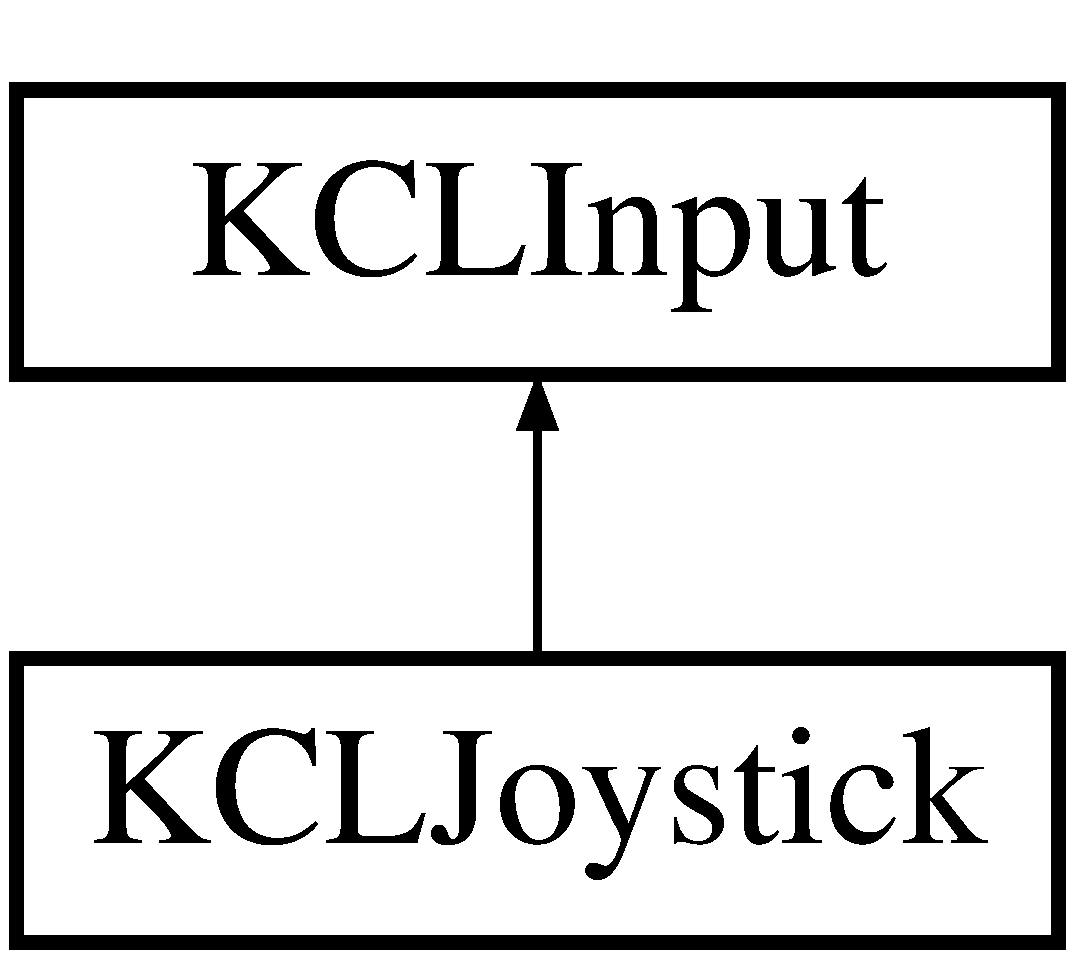
\includegraphics[height=2cm]{class_k_c_l_joystick}
\end{center}
\end{figure}
\subsection*{Public Member Functions}
\begin{CompactItemize}
\item 
\hyperlink{class_k_c_l_joystick_9a424984a46254d07b3ab6b6f5946830}{KCLJoystick} (const QString \&device, QObject $\ast$parent=0)
\item 
int \hyperlink{class_k_c_l_joystick_70988b3702bf410f86a66fb1277913fd}{axisX} ()
\item 
int \hyperlink{class_k_c_l_joystick_0055ef283714ae8545021761e2903376}{axisY} ()
\end{CompactItemize}


\subsection{Constructor \& Destructor Documentation}
\hypertarget{class_k_c_l_joystick_9a424984a46254d07b3ab6b6f5946830}{
\index{KCLJoystick@{KCLJoystick}!KCLJoystick@{KCLJoystick}}
\index{KCLJoystick@{KCLJoystick}!KCLJoystick@{KCLJoystick}}
\subsubsection[{KCLJoystick}]{\setlength{\rightskip}{0pt plus 5cm}KCLJoystick::KCLJoystick (const QString \& {\em device}, \/  QObject $\ast$ {\em parent} = {\tt 0})}}
\label{class_k_c_l_joystick_9a424984a46254d07b3ab6b6f5946830}




\subsection{Member Function Documentation}
\hypertarget{class_k_c_l_joystick_70988b3702bf410f86a66fb1277913fd}{
\index{KCLJoystick@{KCLJoystick}!axisX@{axisX}}
\index{axisX@{axisX}!KCLJoystick@{KCLJoystick}}
\subsubsection[{axisX}]{\setlength{\rightskip}{0pt plus 5cm}int KCLJoystick::axisX ()\hspace{0.3cm}{\tt  \mbox{[}inline\mbox{]}}}}
\label{class_k_c_l_joystick_70988b3702bf410f86a66fb1277913fd}


\hypertarget{class_k_c_l_joystick_0055ef283714ae8545021761e2903376}{
\index{KCLJoystick@{KCLJoystick}!axisY@{axisY}}
\index{axisY@{axisY}!KCLJoystick@{KCLJoystick}}
\subsubsection[{axisY}]{\setlength{\rightskip}{0pt plus 5cm}int KCLJoystick::axisY ()\hspace{0.3cm}{\tt  \mbox{[}inline\mbox{]}}}}
\label{class_k_c_l_joystick_0055ef283714ae8545021761e2903376}




The documentation for this class was generated from the following files:\begin{CompactItemize}
\item 
/home/sacha/programmation/gluon/kcl/\hyperlink{kcljoystick_8h}{kcljoystick.h}\item 
/home/sacha/programmation/gluon/kcl/\hyperlink{kcljoystick_8cpp}{kcljoystick.cpp}\end{CompactItemize}

\hypertarget{class_k_c_l_key_board}{
\section{KCLKeyBoard Class Reference}
\label{class_k_c_l_key_board}\index{KCLKeyBoard@{KCLKeyBoard}}
}
{\tt \#include $<$kclkeyboard.h$>$}

Inheritance diagram for KCLKeyBoard::\begin{figure}[H]
\begin{center}
\leavevmode
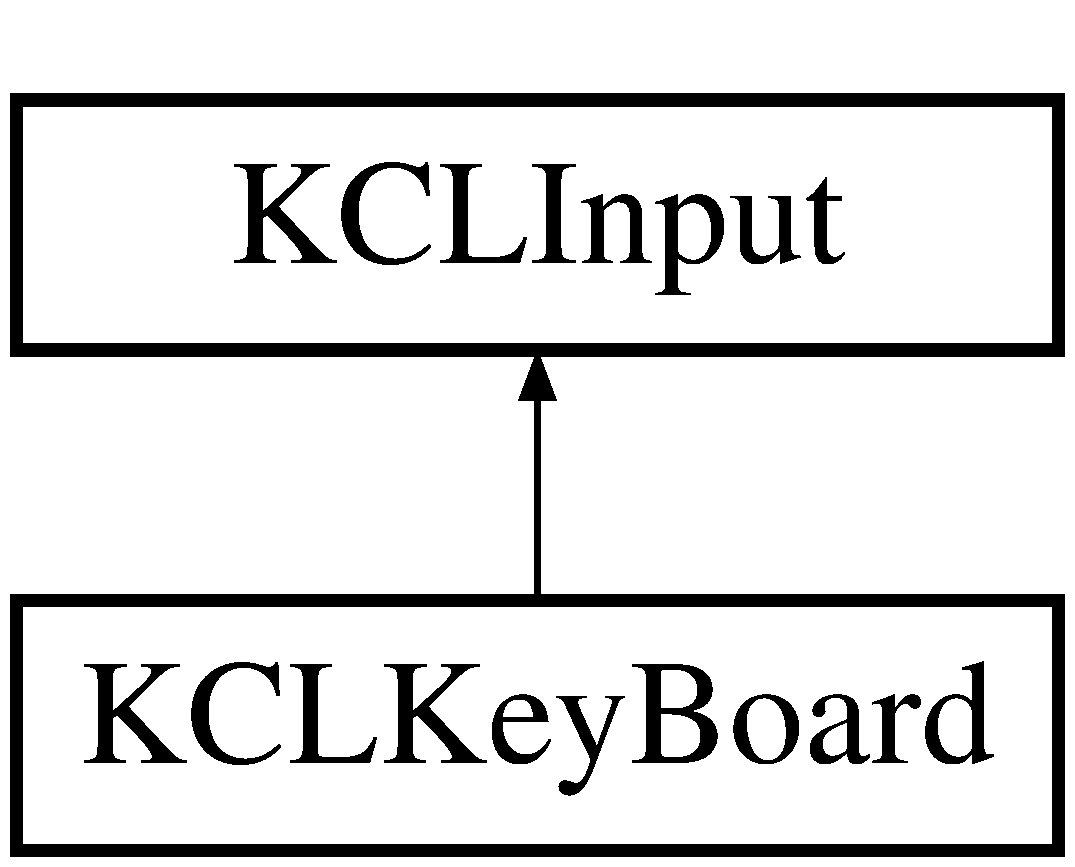
\includegraphics[height=2cm]{class_k_c_l_key_board}
\end{center}
\end{figure}
\subsection*{Public Member Functions}
\begin{CompactItemize}
\item 
\hyperlink{class_k_c_l_key_board_55dbaf0902598d80c7ae60408b47725a}{KCLKeyBoard} (const QString \&device, QObject $\ast$parent=0)
\end{CompactItemize}


\subsection{Constructor \& Destructor Documentation}
\hypertarget{class_k_c_l_key_board_55dbaf0902598d80c7ae60408b47725a}{
\index{KCLKeyBoard@{KCLKeyBoard}!KCLKeyBoard@{KCLKeyBoard}}
\index{KCLKeyBoard@{KCLKeyBoard}!KCLKeyBoard@{KCLKeyBoard}}
\subsubsection[{KCLKeyBoard}]{\setlength{\rightskip}{0pt plus 5cm}KCLKeyBoard::KCLKeyBoard (const QString \& {\em device}, \/  QObject $\ast$ {\em parent} = {\tt 0})}}
\label{class_k_c_l_key_board_55dbaf0902598d80c7ae60408b47725a}




The documentation for this class was generated from the following files:\begin{CompactItemize}
\item 
/home/sacha/programmation/gluon/kcl/\hyperlink{kclkeyboard_8h}{kclkeyboard.h}\item 
/home/sacha/programmation/gluon/kcl/\hyperlink{kclkeyboard_8cpp}{kclkeyboard.cpp}\end{CompactItemize}

\hypertarget{class_k_c_l_mouse}{
\section{KCLMouse Class Reference}
\label{class_k_c_l_mouse}\index{KCLMouse@{KCLMouse}}
}
{\tt \#include $<$kclmouse.h$>$}

Inheritance diagram for KCLMouse::\begin{figure}[H]
\begin{center}
\leavevmode
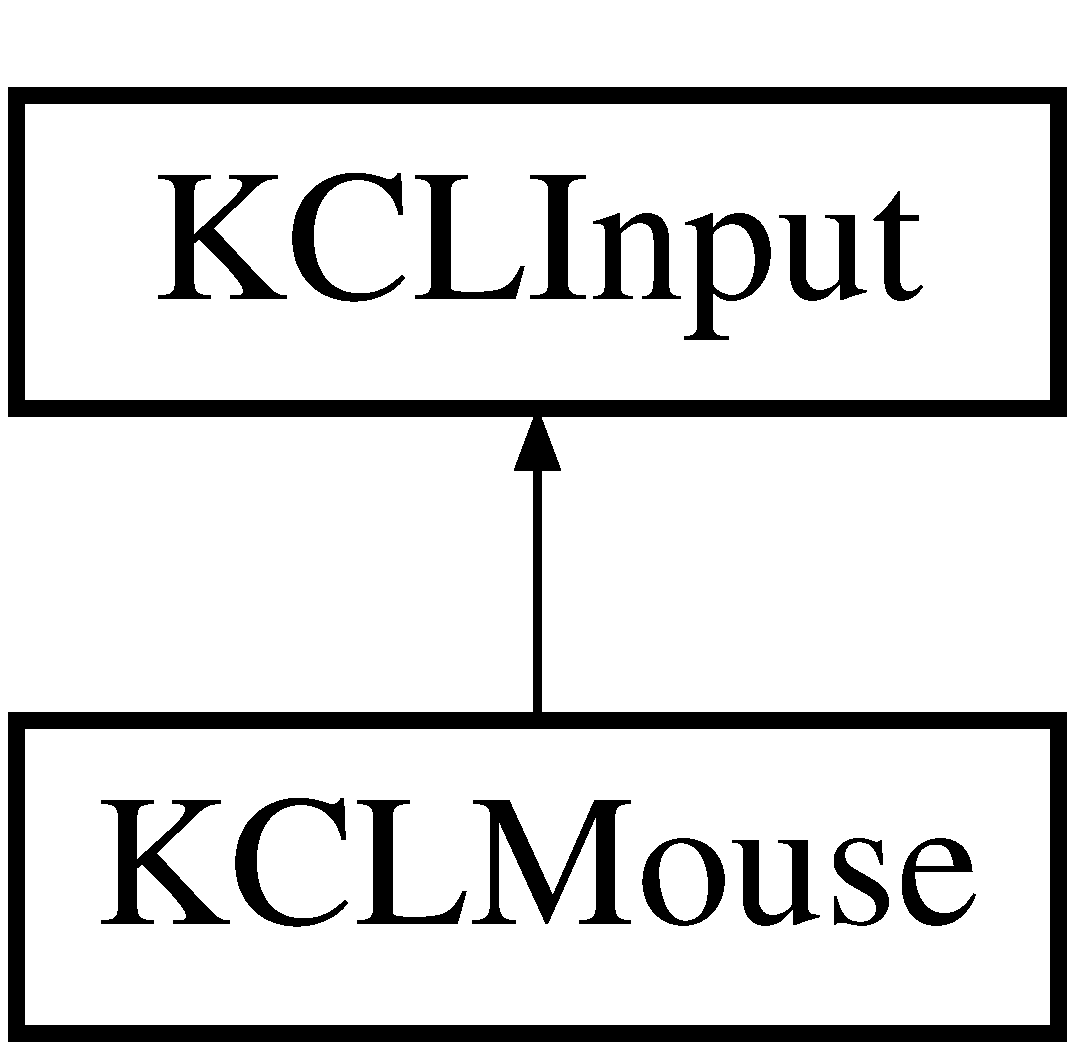
\includegraphics[height=2cm]{class_k_c_l_mouse}
\end{center}
\end{figure}
\subsection*{Public Member Functions}
\begin{CompactItemize}
\item 
\hyperlink{class_k_c_l_mouse_b06e2fabbfd2459d9c335f3dc498f53b}{KCLMouse} (QString device, QObject $\ast$parent=0)
\item 
QPoint \hyperlink{class_k_c_l_mouse_0385a723fb0ec739f8943627764a53fb}{position} ()
\item 
int \hyperlink{class_k_c_l_mouse_a913b0b518584db62a341ad75ee49119}{wheelPosition} ()
\item 
int \hyperlink{class_k_c_l_mouse_75f221554270e5bcffdf6b671a62f01a}{hWheelPosition} ()
\end{CompactItemize}


\subsection{Constructor \& Destructor Documentation}
\hypertarget{class_k_c_l_mouse_b06e2fabbfd2459d9c335f3dc498f53b}{
\index{KCLMouse@{KCLMouse}!KCLMouse@{KCLMouse}}
\index{KCLMouse@{KCLMouse}!KCLMouse@{KCLMouse}}
\subsubsection[{KCLMouse}]{\setlength{\rightskip}{0pt plus 5cm}KCLMouse::KCLMouse (QString {\em device}, \/  QObject $\ast$ {\em parent} = {\tt 0})}}
\label{class_k_c_l_mouse_b06e2fabbfd2459d9c335f3dc498f53b}




\subsection{Member Function Documentation}
\hypertarget{class_k_c_l_mouse_75f221554270e5bcffdf6b671a62f01a}{
\index{KCLMouse@{KCLMouse}!hWheelPosition@{hWheelPosition}}
\index{hWheelPosition@{hWheelPosition}!KCLMouse@{KCLMouse}}
\subsubsection[{hWheelPosition}]{\setlength{\rightskip}{0pt plus 5cm}int KCLMouse::hWheelPosition ()\hspace{0.3cm}{\tt  \mbox{[}inline\mbox{]}}}}
\label{class_k_c_l_mouse_75f221554270e5bcffdf6b671a62f01a}


\hypertarget{class_k_c_l_mouse_0385a723fb0ec739f8943627764a53fb}{
\index{KCLMouse@{KCLMouse}!position@{position}}
\index{position@{position}!KCLMouse@{KCLMouse}}
\subsubsection[{position}]{\setlength{\rightskip}{0pt plus 5cm}QPoint KCLMouse::position ()\hspace{0.3cm}{\tt  \mbox{[}inline\mbox{]}}}}
\label{class_k_c_l_mouse_0385a723fb0ec739f8943627764a53fb}


\hypertarget{class_k_c_l_mouse_a913b0b518584db62a341ad75ee49119}{
\index{KCLMouse@{KCLMouse}!wheelPosition@{wheelPosition}}
\index{wheelPosition@{wheelPosition}!KCLMouse@{KCLMouse}}
\subsubsection[{wheelPosition}]{\setlength{\rightskip}{0pt plus 5cm}int KCLMouse::wheelPosition ()\hspace{0.3cm}{\tt  \mbox{[}inline\mbox{]}}}}
\label{class_k_c_l_mouse_a913b0b518584db62a341ad75ee49119}




The documentation for this class was generated from the following files:\begin{CompactItemize}
\item 
/home/sacha/programmation/gluon/kcl/\hyperlink{kclmouse_8h}{kclmouse.h}\item 
/home/sacha/programmation/gluon/kcl/\hyperlink{kclmouse_8cpp}{kclmouse.cpp}\end{CompactItemize}

\hypertarget{class_k_c_l_thread}{
\section{KCLThread Class Reference}
\label{class_k_c_l_thread}\index{KCLThread@{KCLThread}}
}
Provides a QThread witch listen the input status.  


{\tt \#include $<$Gluon/KCL/KCLInput$>$}

\subsection*{Signals}
\begin{CompactItemize}
\item 
void \hyperlink{class_k_c_l_thread_318807205f19ec5cfbeee2200dbbf995}{emitInputEvent} (\hyperlink{class_k_c_l_input_event}{KCLInputEvent} $\ast$event)
\end{CompactItemize}
\subsection*{Public Member Functions}
\begin{CompactItemize}
\item 
\hyperlink{class_k_c_l_thread_233c3ccb8211c3c247acc7afa3d13381}{KCLThread} (const QString \&name, QObject $\ast$parent=0)
\item 
\hyperlink{class_k_c_l_thread_346cf94ab107d40c2b39d41ff5de6f89}{$\sim$KCLThread} ()
\item 
virtual void \hyperlink{class_k_c_l_thread_12a55f25353d1ba81fc237a1c9dc22b5}{run} ()
\end{CompactItemize}
\subsection*{Protected Member Functions}
\begin{CompactItemize}
\item 
bool \hyperlink{class_k_c_l_thread_2b5d9cafcdbbf26ceac9cc9cce9427dc}{openDevice} (const QString \&device)
\item 
void \hyperlink{class_k_c_l_thread_dc58b5a20a35371ecf539c51098411c6}{closeDevice} ()
\end{CompactItemize}


\subsection{Detailed Description}
Provides a QThread witch listen the input status. 

\begin{Desc}
\item[Author:]sacha schutz $<$\href{mailto:istdasklar@gmail.com}{\tt istdasklar@gmail.com}$>$ \end{Desc}


\subsection{Constructor \& Destructor Documentation}
\hypertarget{class_k_c_l_thread_233c3ccb8211c3c247acc7afa3d13381}{
\index{KCLThread@{KCLThread}!KCLThread@{KCLThread}}
\index{KCLThread@{KCLThread}!KCLThread@{KCLThread}}
\subsubsection[{KCLThread}]{\setlength{\rightskip}{0pt plus 5cm}KCLThread::KCLThread (const QString \& {\em name}, \/  QObject $\ast$ {\em parent} = {\tt 0})}}
\label{class_k_c_l_thread_233c3ccb8211c3c247acc7afa3d13381}


\hypertarget{class_k_c_l_thread_346cf94ab107d40c2b39d41ff5de6f89}{
\index{KCLThread@{KCLThread}!$\sim$KCLThread@{$\sim$KCLThread}}
\index{$\sim$KCLThread@{$\sim$KCLThread}!KCLThread@{KCLThread}}
\subsubsection[{$\sim$KCLThread}]{\setlength{\rightskip}{0pt plus 5cm}KCLThread::$\sim$KCLThread ()\hspace{0.3cm}{\tt  \mbox{[}inline\mbox{]}}}}
\label{class_k_c_l_thread_346cf94ab107d40c2b39d41ff5de6f89}




\subsection{Member Function Documentation}
\hypertarget{class_k_c_l_thread_dc58b5a20a35371ecf539c51098411c6}{
\index{KCLThread@{KCLThread}!closeDevice@{closeDevice}}
\index{closeDevice@{closeDevice}!KCLThread@{KCLThread}}
\subsubsection[{closeDevice}]{\setlength{\rightskip}{0pt plus 5cm}void KCLThread::closeDevice ()\hspace{0.3cm}{\tt  \mbox{[}inline, protected\mbox{]}}}}
\label{class_k_c_l_thread_dc58b5a20a35371ecf539c51098411c6}


\hypertarget{class_k_c_l_thread_318807205f19ec5cfbeee2200dbbf995}{
\index{KCLThread@{KCLThread}!emitInputEvent@{emitInputEvent}}
\index{emitInputEvent@{emitInputEvent}!KCLThread@{KCLThread}}
\subsubsection[{emitInputEvent}]{\setlength{\rightskip}{0pt plus 5cm}void KCLThread::emitInputEvent ({\bf KCLInputEvent} $\ast$ {\em event})\hspace{0.3cm}{\tt  \mbox{[}signal\mbox{]}}}}
\label{class_k_c_l_thread_318807205f19ec5cfbeee2200dbbf995}


emit a \hyperlink{class_k_c_l_input}{KCLInput}. This signal is emited when somthing happen on a device. \hypertarget{class_k_c_l_thread_2b5d9cafcdbbf26ceac9cc9cce9427dc}{
\index{KCLThread@{KCLThread}!openDevice@{openDevice}}
\index{openDevice@{openDevice}!KCLThread@{KCLThread}}
\subsubsection[{openDevice}]{\setlength{\rightskip}{0pt plus 5cm}bool KCLThread::openDevice (const QString \& {\em device})\hspace{0.3cm}{\tt  \mbox{[}protected\mbox{]}}}}
\label{class_k_c_l_thread_2b5d9cafcdbbf26ceac9cc9cce9427dc}


\hypertarget{class_k_c_l_thread_12a55f25353d1ba81fc237a1c9dc22b5}{
\index{KCLThread@{KCLThread}!run@{run}}
\index{run@{run}!KCLThread@{KCLThread}}
\subsubsection[{run}]{\setlength{\rightskip}{0pt plus 5cm}void KCLThread::run ()\hspace{0.3cm}{\tt  \mbox{[}virtual\mbox{]}}}}
\label{class_k_c_l_thread_12a55f25353d1ba81fc237a1c9dc22b5}




The documentation for this class was generated from the following files:\begin{CompactItemize}
\item 
/home/sacha/programmation/gluon/kcl/\hyperlink{kclinput_8h}{kclinput.h}\item 
/home/sacha/programmation/gluon/kcl/\hyperlink{kclinput_8cpp}{kclinput.cpp}\end{CompactItemize}

\hypertarget{class_virtual_button}{
\section{VirtualButton Class Reference}
\label{class_virtual_button}\index{VirtualButton@{VirtualButton}}
}
{\tt \#include $<$kclvirtualinput.h$>$}

\subsection*{Public Member Functions}
\begin{CompactItemize}
\item 
\hyperlink{class_virtual_button_446757ea5603b9d9bd90391d31a7de98}{VirtualButton} (QString name=0, int buttonCode=0, \hyperlink{class_k_c_l_input}{KCLInput} $\ast$input=NULL)
\item 
QString \hyperlink{class_virtual_button_6a5bdaf694c545e88225f9aff3a89d78}{name} ()
\item 
int \hyperlink{class_virtual_button_807d21790a5cfa564b1e20d28f900051}{code} ()
\item 
\hyperlink{class_k_c_l_input}{KCLInput} $\ast$ \hyperlink{class_virtual_button_1c67f8dec41ff21d0aa5c07225771e07}{input} ()
\item 
void \hyperlink{class_virtual_button_f66cc874223da73e9e68f05f4470a2a1}{setName} (const QString \&name)
\item 
void \hyperlink{class_virtual_button_fb49f0be2e423669ed4ef30e2d4c11a4}{setButtonCode} (int code)
\item 
void \hyperlink{class_virtual_button_08f64dcc90e220b3ff9720f2cdf29072}{setInput} (\hyperlink{class_k_c_l_input}{KCLInput} $\ast$input)
\end{CompactItemize}


\subsection{Constructor \& Destructor Documentation}
\hypertarget{class_virtual_button_446757ea5603b9d9bd90391d31a7de98}{
\index{VirtualButton@{VirtualButton}!VirtualButton@{VirtualButton}}
\index{VirtualButton@{VirtualButton}!VirtualButton@{VirtualButton}}
\subsubsection[{VirtualButton}]{\setlength{\rightskip}{0pt plus 5cm}VirtualButton::VirtualButton (QString {\em name} = {\tt 0}, \/  int {\em buttonCode} = {\tt 0}, \/  {\bf KCLInput} $\ast$ {\em input} = {\tt NULL})}}
\label{class_virtual_button_446757ea5603b9d9bd90391d31a7de98}




\subsection{Member Function Documentation}
\hypertarget{class_virtual_button_807d21790a5cfa564b1e20d28f900051}{
\index{VirtualButton@{VirtualButton}!code@{code}}
\index{code@{code}!VirtualButton@{VirtualButton}}
\subsubsection[{code}]{\setlength{\rightskip}{0pt plus 5cm}int VirtualButton::code ()\hspace{0.3cm}{\tt  \mbox{[}inline\mbox{]}}}}
\label{class_virtual_button_807d21790a5cfa564b1e20d28f900051}


\hypertarget{class_virtual_button_1c67f8dec41ff21d0aa5c07225771e07}{
\index{VirtualButton@{VirtualButton}!input@{input}}
\index{input@{input}!VirtualButton@{VirtualButton}}
\subsubsection[{input}]{\setlength{\rightskip}{0pt plus 5cm}{\bf KCLInput}$\ast$ VirtualButton::input ()\hspace{0.3cm}{\tt  \mbox{[}inline\mbox{]}}}}
\label{class_virtual_button_1c67f8dec41ff21d0aa5c07225771e07}


\hypertarget{class_virtual_button_6a5bdaf694c545e88225f9aff3a89d78}{
\index{VirtualButton@{VirtualButton}!name@{name}}
\index{name@{name}!VirtualButton@{VirtualButton}}
\subsubsection[{name}]{\setlength{\rightskip}{0pt plus 5cm}QString VirtualButton::name ()\hspace{0.3cm}{\tt  \mbox{[}inline\mbox{]}}}}
\label{class_virtual_button_6a5bdaf694c545e88225f9aff3a89d78}


\hypertarget{class_virtual_button_fb49f0be2e423669ed4ef30e2d4c11a4}{
\index{VirtualButton@{VirtualButton}!setButtonCode@{setButtonCode}}
\index{setButtonCode@{setButtonCode}!VirtualButton@{VirtualButton}}
\subsubsection[{setButtonCode}]{\setlength{\rightskip}{0pt plus 5cm}void VirtualButton::setButtonCode (int {\em code})\hspace{0.3cm}{\tt  \mbox{[}inline\mbox{]}}}}
\label{class_virtual_button_fb49f0be2e423669ed4ef30e2d4c11a4}


\hypertarget{class_virtual_button_08f64dcc90e220b3ff9720f2cdf29072}{
\index{VirtualButton@{VirtualButton}!setInput@{setInput}}
\index{setInput@{setInput}!VirtualButton@{VirtualButton}}
\subsubsection[{setInput}]{\setlength{\rightskip}{0pt plus 5cm}void VirtualButton::setInput ({\bf KCLInput} $\ast$ {\em input})\hspace{0.3cm}{\tt  \mbox{[}inline\mbox{]}}}}
\label{class_virtual_button_08f64dcc90e220b3ff9720f2cdf29072}


\hypertarget{class_virtual_button_f66cc874223da73e9e68f05f4470a2a1}{
\index{VirtualButton@{VirtualButton}!setName@{setName}}
\index{setName@{setName}!VirtualButton@{VirtualButton}}
\subsubsection[{setName}]{\setlength{\rightskip}{0pt plus 5cm}void VirtualButton::setName (const QString \& {\em name})\hspace{0.3cm}{\tt  \mbox{[}inline\mbox{]}}}}
\label{class_virtual_button_f66cc874223da73e9e68f05f4470a2a1}




The documentation for this class was generated from the following files:\begin{CompactItemize}
\item 
/home/sacha/programmation/gluon/kcl/\hyperlink{kclvirtualinput_8h}{kclvirtualinput.h}\item 
/home/sacha/programmation/gluon/kcl/\hyperlink{kclvirtualinput_8cpp}{kclvirtualinput.cpp}\end{CompactItemize}

\chapter{File Documentation}
\hypertarget{kclcode_8cpp}{
\section{/home/sacha/programmation/gluon/kcl/kclcode.cpp File Reference}
\label{kclcode_8cpp}\index{/home/sacha/programmation/gluon/kcl/kclcode.cpp@{/home/sacha/programmation/gluon/kcl/kclcode.cpp}}
}
{\tt \#include \char`\"{}kclcode.h\char`\"{}}\par
{\tt \#include $<$linux/input.h$>$}\par
{\tt \#include $<$linux/version.h$>$}\par
{\tt \#include $<$string.h$>$}\par
{\tt \#include $<$fcntl.h$>$}\par
{\tt \#include $<$unistd.h$>$}\par
{\tt \#include $<$stdlib.h$>$}\par
{\tt \#include $<$stdio.h$>$}\par
\subsection*{Variables}
\begin{CompactItemize}
\item 
const char $\ast$ \hyperlink{kclcode_8cpp_38ff2e09331936124b4be0f6da2003e4}{KCL\_\-CODE\_\-EVENT} \mbox{[}EV\_\-MAX+1\mbox{]}
\item 
const char $\ast$ \hyperlink{kclcode_8cpp_935cf139ace4d8a7280a71b33e785216}{KCL\_\-CODE\_\-BUTTON} \mbox{[}KEY\_\-MAX+1\mbox{]}
\item 
const char $\ast$ \hyperlink{kclcode_8cpp_cb5307a02c57fb0ba60741f40241a743}{KCL\_\-CODE\_\-RELATIV} \mbox{[}REL\_\-MAX+1\mbox{]}
\item 
const char $\ast$ \hyperlink{kclcode_8cpp_603b96aa9f906ba85183cd89d8e5e5d7}{KCL\_\-CODE\_\-ABSOLU} \mbox{[}ABS\_\-MAX+1\mbox{]}
\end{CompactItemize}


\subsection{Variable Documentation}
\hypertarget{kclcode_8cpp_603b96aa9f906ba85183cd89d8e5e5d7}{
\index{kclcode.cpp@{kclcode.cpp}!KCL\_\-CODE\_\-ABSOLU@{KCL\_\-CODE\_\-ABSOLU}}
\index{KCL\_\-CODE\_\-ABSOLU@{KCL\_\-CODE\_\-ABSOLU}!kclcode.cpp@{kclcode.cpp}}
\subsubsection[{KCL\_\-CODE\_\-ABSOLU}]{\setlength{\rightskip}{0pt plus 5cm}const char$\ast$ {\bf KCL\_\-CODE\_\-ABSOLU}\mbox{[}ABS\_\-MAX+1\mbox{]}}}
\label{kclcode_8cpp_603b96aa9f906ba85183cd89d8e5e5d7}


\textbf{Initial value:}

\begin{Code}\begin{verbatim}
          { "X", "Y", "Z", "Rx",  "Ry", "Rz", "Throttle", "Rudder",
            "Wheel", "Gas", "Brake", NULL, NULL, NULL, NULL, NULL,
             "Hat0X", "Hat0Y", "Hat1X", "Hat1Y",
            "Hat2X", "Hat2Y", "Hat3X", "Hat 3Y",
            "Pressure", "Distance", "XTilt", "YTilt",
            "ToolWidth", NULL, NULL, NULL,
             "Volume", NULL, NULL, NULL,
            NULL, NULL, NULL, NULL,
             "Misc" }
\end{verbatim}
\end{Code}
\hypertarget{kclcode_8cpp_935cf139ace4d8a7280a71b33e785216}{
\index{kclcode.cpp@{kclcode.cpp}!KCL\_\-CODE\_\-BUTTON@{KCL\_\-CODE\_\-BUTTON}}
\index{KCL\_\-CODE\_\-BUTTON@{KCL\_\-CODE\_\-BUTTON}!kclcode.cpp@{kclcode.cpp}}
\subsubsection[{KCL\_\-CODE\_\-BUTTON}]{\setlength{\rightskip}{0pt plus 5cm}const char$\ast$ {\bf KCL\_\-CODE\_\-BUTTON}\mbox{[}KEY\_\-MAX+1\mbox{]}}}
\label{kclcode_8cpp_935cf139ace4d8a7280a71b33e785216}


\hypertarget{kclcode_8cpp_38ff2e09331936124b4be0f6da2003e4}{
\index{kclcode.cpp@{kclcode.cpp}!KCL\_\-CODE\_\-EVENT@{KCL\_\-CODE\_\-EVENT}}
\index{KCL\_\-CODE\_\-EVENT@{KCL\_\-CODE\_\-EVENT}!kclcode.cpp@{kclcode.cpp}}
\subsubsection[{KCL\_\-CODE\_\-EVENT}]{\setlength{\rightskip}{0pt plus 5cm}const char$\ast$ {\bf KCL\_\-CODE\_\-EVENT}\mbox{[}EV\_\-MAX+1\mbox{]}}}
\label{kclcode_8cpp_38ff2e09331936124b4be0f6da2003e4}


\textbf{Initial value:}

\begin{Code}\begin{verbatim} { "Reset", "Key", "Relative", "Absolute", "MSC", NULL, NULL, NULL, NULL, NULL, NULL, NULL, NULL, NULL,
        NULL, NULL, NULL, "LED", "Sound", NULL, "Repeat", "ForceFeedback", "Power", "ForceFeedbackStatus"}
\end{verbatim}
\end{Code}
\hypertarget{kclcode_8cpp_cb5307a02c57fb0ba60741f40241a743}{
\index{kclcode.cpp@{kclcode.cpp}!KCL\_\-CODE\_\-RELATIV@{KCL\_\-CODE\_\-RELATIV}}
\index{KCL\_\-CODE\_\-RELATIV@{KCL\_\-CODE\_\-RELATIV}!kclcode.cpp@{kclcode.cpp}}
\subsubsection[{KCL\_\-CODE\_\-RELATIV}]{\setlength{\rightskip}{0pt plus 5cm}const char$\ast$ {\bf KCL\_\-CODE\_\-RELATIV}\mbox{[}REL\_\-MAX+1\mbox{]}}}
\label{kclcode_8cpp_cb5307a02c57fb0ba60741f40241a743}


\textbf{Initial value:}

\begin{Code}\begin{verbatim}
          { "X", "Y", "Z", NULL,
            NULL, NULL, "HWheel", "Dial",
             "Wheel", "MISC" }
\end{verbatim}
\end{Code}

\hypertarget{kclcode_8h}{
\section{/home/sacha/programmation/gluon/kcl/kclcode.h File Reference}
\label{kclcode_8h}\index{/home/sacha/programmation/gluon/kcl/kclcode.h@{/home/sacha/programmation/gluon/kcl/kclcode.h}}
}
{\tt \#include $<$QString$>$}\par
\subsection*{Classes}
\begin{CompactItemize}
\item 
class \hyperlink{class_k_c_l_code}{KCLCode}
\end{CompactItemize}

\hypertarget{kcldevicemodel_8cpp}{
\section{/home/sacha/programmation/gluon/kcl/kcldevicemodel.cpp File Reference}
\label{kcldevicemodel_8cpp}\index{/home/sacha/programmation/gluon/kcl/kcldevicemodel.cpp@{/home/sacha/programmation/gluon/kcl/kcldevicemodel.cpp}}
}
{\tt \#include \char`\"{}kcldevicemodel.h\char`\"{}}\par
{\tt \#include $<$KIcon$>$}\par
{\tt \#include $<$KDebug$>$}\par
{\tt \#include $<$QMessageBox$>$}\par

\hypertarget{kcldevicemodel_8h}{
\section{/home/sacha/programmation/gluon/kcl/kcldevicemodel.h File Reference}
\label{kcldevicemodel_8h}\index{/home/sacha/programmation/gluon/kcl/kcldevicemodel.h@{/home/sacha/programmation/gluon/kcl/kcldevicemodel.h}}
}
{\tt \#include $<$QStandardItemModel$>$}\par
{\tt \#include $<$KIcon$>$}\par
{\tt \#include \char`\"{}kclengine.h\char`\"{}}\par
\subsection*{Classes}
\begin{CompactItemize}
\item 
class \hyperlink{class_k_c_l_device_model}{KCLDeviceModel}
\end{CompactItemize}

\hypertarget{kclengine_8cpp}{
\section{/home/sacha/programmation/gluon/kcl/kclengine.cpp File Reference}
\label{kclengine_8cpp}\index{/home/sacha/programmation/gluon/kcl/kclengine.cpp@{/home/sacha/programmation/gluon/kcl/kclengine.cpp}}
}
{\tt \#include \char`\"{}kclengine.h\char`\"{}}\par
{\tt \#include $<$KDebug$>$}\par
{\tt \#include $<$QApplication$>$}\par
{\tt \#include $<$QFile$>$}\par
{\tt \#include $<$QDir$>$}\par

\hypertarget{kclengine_8h}{
\section{/home/sacha/programmation/gluon/kcl/kclengine.h File Reference}
\label{kclengine_8h}\index{/home/sacha/programmation/gluon/kcl/kclengine.h@{/home/sacha/programmation/gluon/kcl/kclengine.h}}
}
{\tt \#include $<$QObject$>$}\par
{\tt \#include $<$QList$>$}\par
{\tt \#include $<$QMap$>$}\par
{\tt \#include $<$QPair$>$}\par
{\tt \#include $<$QStringList$>$}\par
{\tt \#include $<$solid/devicenotifier.h$>$}\par
{\tt \#include $<$solid/device.h$>$}\par
{\tt \#include $<$kcomponentdata.h$>$}\par
{\tt \#include \char`\"{}kclinput.h\char`\"{}}\par
{\tt \#include \char`\"{}kclmouse.h\char`\"{}}\par
{\tt \#include \char`\"{}kcljoystick.h\char`\"{}}\par
{\tt \#include \char`\"{}kclkeyboard.h\char`\"{}}\par
\subsection*{Classes}
\begin{CompactItemize}
\item 
class \hyperlink{class_virtual_button}{VirtualButton}
\item 
class \hyperlink{class_k_c_l_engine}{KCLEngine}
\end{CompactItemize}

\hypertarget{kclinfowidget_8cpp}{
\section{/home/sacha/programmation/gluon/kcl/kclinfowidget.cpp File Reference}
\label{kclinfowidget_8cpp}\index{/home/sacha/programmation/gluon/kcl/kclinfowidget.cpp@{/home/sacha/programmation/gluon/kcl/kclinfowidget.cpp}}
}
{\tt \#include \char`\"{}kclinfowidget.h\char`\"{}}\par
{\tt \#include $<$QVBoxLayout$>$}\par
{\tt \#include $<$KIcon$>$}\par
{\tt \#include $<$KPushButton$>$}\par
{\tt \#include $<$QLabel$>$}\par
{\tt \#include $<$KLocale$>$}\par
{\tt \#include $<$QProcess$>$}\par
{\tt \#include $<$KMessageBox$>$}\par
{\tt \#include $<$QGroupBox$>$}\par
{\tt \#include $<$KSeparator$>$}\par

\hypertarget{kclinfowidget_8h}{
\section{/home/sacha/programmation/gluon/kcl/kclinfowidget.h File Reference}
\label{kclinfowidget_8h}\index{/home/sacha/programmation/gluon/kcl/kclinfowidget.h@{/home/sacha/programmation/gluon/kcl/kclinfowidget.h}}
}
{\tt \#include $<$QWidget$>$}\par
{\tt \#include $<$KTitleWidget$>$}\par
{\tt \#include $<$QLabel$>$}\par
{\tt \#include $<$KTabWidget$>$}\par
{\tt \#include $<$QTreeView$>$}\par
{\tt \#include $<$QGraphicsView$>$}\par
{\tt \#include \char`\"{}kcldevicemodel.h\char`\"{}}\par
{\tt \#include \char`\"{}kclbutton.h\char`\"{}}\par
\subsection*{Classes}
\begin{CompactItemize}
\item 
class \hyperlink{class_k_c_l_info_widget}{KCLInfoWidget}
\end{CompactItemize}

\hypertarget{kclinput_8cpp}{
\section{/home/sacha/programmation/gluon/kcl/kclinput.cpp File Reference}
\label{kclinput_8cpp}\index{/home/sacha/programmation/gluon/kcl/kclinput.cpp@{/home/sacha/programmation/gluon/kcl/kclinput.cpp}}
}
{\tt \#include \char`\"{}kclinput.h\char`\"{}}\par
{\tt \#include $<$KDebug$>$}\par
{\tt \#include $<$QFile$>$}\par
{\tt \#include $<$QMessageBox$>$}\par
\subsection*{Defines}
\begin{CompactItemize}
\item 
\#define \hyperlink{kclinput_8cpp_2f660aa23a5dbc0f4b8df48b4302b8c3}{BITS\_\-PER\_\-LONG}~(sizeof(long) $\ast$ 8)
\item 
\#define \hyperlink{kclinput_8cpp_1f296f3f5ec473b603ee32e2f7577fcb}{NBITS}(x)~((((x)-1)/BITS\_\-PER\_\-LONG)+1)
\item 
\#define \hyperlink{kclinput_8cpp_4521467edec9387fad3ae8761f0f4b1d}{OFF}(x)~((x)\%BITS\_\-PER\_\-LONG)
\item 
\#define \hyperlink{kclinput_8cpp_d27cc17b25bb93134368d5eb21126eae}{BIT}(x)~(1UL$<$$<$OFF(x))
\item 
\#define \hyperlink{kclinput_8cpp_f647a68a4985fd16c40d533b0ab21bac}{LONG}(x)~((x)/BITS\_\-PER\_\-LONG)
\item 
\#define \hyperlink{kclinput_8cpp_9bfbfcfdf94e66aad3e5113c5acf4072}{test\_\-bit}(bit, array)~((array\mbox{[}LONG(bit)\mbox{]} $>$$>$ OFF(bit)) \& 1)
\end{CompactItemize}


\subsection{Define Documentation}
\hypertarget{kclinput_8cpp_d27cc17b25bb93134368d5eb21126eae}{
\index{kclinput.cpp@{kclinput.cpp}!BIT@{BIT}}
\index{BIT@{BIT}!kclinput.cpp@{kclinput.cpp}}
\subsubsection[{BIT}]{\setlength{\rightskip}{0pt plus 5cm}\#define BIT(x)~(1UL$<$$<$OFF(x))}}
\label{kclinput_8cpp_d27cc17b25bb93134368d5eb21126eae}


\hypertarget{kclinput_8cpp_2f660aa23a5dbc0f4b8df48b4302b8c3}{
\index{kclinput.cpp@{kclinput.cpp}!BITS\_\-PER\_\-LONG@{BITS\_\-PER\_\-LONG}}
\index{BITS\_\-PER\_\-LONG@{BITS\_\-PER\_\-LONG}!kclinput.cpp@{kclinput.cpp}}
\subsubsection[{BITS\_\-PER\_\-LONG}]{\setlength{\rightskip}{0pt plus 5cm}\#define BITS\_\-PER\_\-LONG~(sizeof(long) $\ast$ 8)}}
\label{kclinput_8cpp_2f660aa23a5dbc0f4b8df48b4302b8c3}


\hypertarget{kclinput_8cpp_f647a68a4985fd16c40d533b0ab21bac}{
\index{kclinput.cpp@{kclinput.cpp}!LONG@{LONG}}
\index{LONG@{LONG}!kclinput.cpp@{kclinput.cpp}}
\subsubsection[{LONG}]{\setlength{\rightskip}{0pt plus 5cm}\#define LONG(x)~((x)/BITS\_\-PER\_\-LONG)}}
\label{kclinput_8cpp_f647a68a4985fd16c40d533b0ab21bac}


\hypertarget{kclinput_8cpp_1f296f3f5ec473b603ee32e2f7577fcb}{
\index{kclinput.cpp@{kclinput.cpp}!NBITS@{NBITS}}
\index{NBITS@{NBITS}!kclinput.cpp@{kclinput.cpp}}
\subsubsection[{NBITS}]{\setlength{\rightskip}{0pt plus 5cm}\#define NBITS(x)~((((x)-1)/BITS\_\-PER\_\-LONG)+1)}}
\label{kclinput_8cpp_1f296f3f5ec473b603ee32e2f7577fcb}


\hypertarget{kclinput_8cpp_4521467edec9387fad3ae8761f0f4b1d}{
\index{kclinput.cpp@{kclinput.cpp}!OFF@{OFF}}
\index{OFF@{OFF}!kclinput.cpp@{kclinput.cpp}}
\subsubsection[{OFF}]{\setlength{\rightskip}{0pt plus 5cm}\#define OFF(x)~((x)\%BITS\_\-PER\_\-LONG)}}
\label{kclinput_8cpp_4521467edec9387fad3ae8761f0f4b1d}


\hypertarget{kclinput_8cpp_9bfbfcfdf94e66aad3e5113c5acf4072}{
\index{kclinput.cpp@{kclinput.cpp}!test\_\-bit@{test\_\-bit}}
\index{test\_\-bit@{test\_\-bit}!kclinput.cpp@{kclinput.cpp}}
\subsubsection[{test\_\-bit}]{\setlength{\rightskip}{0pt plus 5cm}\#define test\_\-bit(bit, \/  array)~((array\mbox{[}LONG(bit)\mbox{]} $>$$>$ OFF(bit)) \& 1)}}
\label{kclinput_8cpp_9bfbfcfdf94e66aad3e5113c5acf4072}



\hypertarget{kclinput_8h}{
\section{/home/sacha/programmation/gluon/kcl/kclinput.h File Reference}
\label{kclinput_8h}\index{/home/sacha/programmation/gluon/kcl/kclinput.h@{/home/sacha/programmation/gluon/kcl/kclinput.h}}
}
{\tt \#include $<$QThread$>$}\par
{\tt \#include $<$QMap$>$}\par
{\tt \#include $<$QPair$>$}\par
{\tt \#include $<$QPoint$>$}\par
{\tt \#include $<$unistd.h$>$}\par
{\tt \#include $<$fcntl.h$>$}\par
{\tt \#include $<$sys/stat.h$>$}\par
{\tt \#include $<$sys/types.h$>$}\par
{\tt \#include $<$stdio.h$>$}\par
{\tt \#include $<$linux/input.h$>$}\par
{\tt \#include $<$KDebug$>$}\par
{\tt \#include \char`\"{}kclcode.h\char`\"{}}\par
{\tt \#include \char`\"{}kcl.h\char`\"{}}\par
\subsection*{Classes}
\begin{CompactItemize}
\item 
class \hyperlink{class_abs_val}{AbsVal}
\item 
class \hyperlink{class_k_c_l_input_event}{KCLInputEvent}
\begin{CompactList}\small\item\em Provides a input events. \item\end{CompactList}\item 
class \hyperlink{class_k_c_l_thread}{KCLThread}
\begin{CompactList}\small\item\em Provides a QThread witch listen the input status. \item\end{CompactList}\item 
class \hyperlink{class_k_c_l_input}{KCLInput}
\begin{CompactList}\small\item\em provide an object that represent an input. This is the class mother of all device you want to use. It return you all information about the device, for example the name. And it return the status of the device, it means the type, code, and value. \item\end{CompactList}\end{CompactItemize}

\hypertarget{kcljoystick_8cpp}{
\section{/home/sacha/programmation/gluon/kcl/kcljoystick.cpp File Reference}
\label{kcljoystick_8cpp}\index{/home/sacha/programmation/gluon/kcl/kcljoystick.cpp@{/home/sacha/programmation/gluon/kcl/kcljoystick.cpp}}
}
{\tt \#include \char`\"{}kcljoystick.h\char`\"{}}\par

\hypertarget{kcljoystick_8h}{
\section{/home/sacha/programmation/gluon/kcl/kcljoystick.h File Reference}
\label{kcljoystick_8h}\index{/home/sacha/programmation/gluon/kcl/kcljoystick.h@{/home/sacha/programmation/gluon/kcl/kcljoystick.h}}
}
{\tt \#include \char`\"{}kclinput.h\char`\"{}}\par
\subsection*{Classes}
\begin{CompactItemize}
\item 
class \hyperlink{class_k_c_l_joystick}{KCLJoystick}
\end{CompactItemize}

\hypertarget{kclkeyboard_8cpp}{
\section{/home/sacha/programmation/gluon/kcl/kclkeyboard.cpp File Reference}
\label{kclkeyboard_8cpp}\index{/home/sacha/programmation/gluon/kcl/kclkeyboard.cpp@{/home/sacha/programmation/gluon/kcl/kclkeyboard.cpp}}
}
{\tt \#include \char`\"{}kclkeyboard.h\char`\"{}}\par
{\tt \#include $<$KDebug$>$}\par

\hypertarget{kclkeyboard_8h}{
\section{/home/sacha/programmation/gluon/kcl/kclkeyboard.h File Reference}
\label{kclkeyboard_8h}\index{/home/sacha/programmation/gluon/kcl/kclkeyboard.h@{/home/sacha/programmation/gluon/kcl/kclkeyboard.h}}
}
{\tt \#include \char`\"{}kclinput.h\char`\"{}}\par
\subsection*{Classes}
\begin{CompactItemize}
\item 
class \hyperlink{class_k_c_l_key_board}{KCLKeyBoard}
\end{CompactItemize}

\hypertarget{kclmouse_8cpp}{
\section{/home/sacha/programmation/gluon/kcl/kclmouse.cpp File Reference}
\label{kclmouse_8cpp}\index{/home/sacha/programmation/gluon/kcl/kclmouse.cpp@{/home/sacha/programmation/gluon/kcl/kclmouse.cpp}}
}
{\tt \#include \char`\"{}kclmouse.h\char`\"{}}\par
{\tt \#include $<$KDebug$>$}\par

\hypertarget{kclmouse_8h}{
\section{/home/sacha/programmation/gluon/kcl/kclmouse.h File Reference}
\label{kclmouse_8h}\index{/home/sacha/programmation/gluon/kcl/kclmouse.h@{/home/sacha/programmation/gluon/kcl/kclmouse.h}}
}
{\tt \#include \char`\"{}kclinput.h\char`\"{}}\par
{\tt \#include $<$QPoint$>$}\par
{\tt \#include $<$QList$>$}\par
{\tt \#include $<$QWidget$>$}\par
\subsection*{Classes}
\begin{CompactItemize}
\item 
class \hyperlink{class_k_c_l_mouse}{KCLMouse}
\end{CompactItemize}

\printindex
\end{document}
